\documentclass[11 pt]{scrartcl}
\usepackage[header, margin, koma, stylish]{tyler}
\usetikzlibrary{automata,arrows,positioning,calc}
\usepackage{csquotes}

\pagestyle{fancy}
\fancyhf{}
\fancyhead[l]{EECS 126 Notes}
\fancyhead[r]{Tyler Zhu}
\cfoot{\thepage}

\newcommand\reflexive[2]{% node, label
  \draw[->] (#1.100) to[reflexive] node[trans,above=-2mm] {#2} (#1.80); 
}
\newcommand\link[3]{% start node, end node, label
  \draw[edge] (#1) -- (#1 |- #2);
  \node[trans] at (#1 |- #2) {#3} (1);
  \draw[edge] (#1 |- #2) -- (#2);
}
\newcommand\linkwithdots[4]{% start node, end node, dots node, label
  \coordinate (dots1) at (#1 |- #3);
  \draw (#1) -- ([yshift=5mm]dots1);
  \draw[dotted] ([yshift=5mm]dots1) -- ([yshift=-5mm]dots1);
  \draw[edge] ([yshift=-5mm]dots1) -- (#1 |- #2);
  \node[trans] at (#1 |- #2) {#4} (1);
  \coordinate (dots2) at (#3 |- #2);
  \draw (#1 |- #2) -- ([xshift=-5mm]dots2);
  \draw[dotted] ([xshift=-5mm]dots2) -- ([xshift=5mm]dots2);
  \draw[edge] ([xshift=5mm]dots2) -- (#2);
}

\begin{document} 
\title{\Large EECS 126 Notes}
\author{\large Tyler Zhu}
\date{\large\today}

\maketitle 

\begin{center}
\begin{displayquote}
    \emph{"A good stock of examples, as large as possible, is indispensable for a thorough understanding of any concept, and when I want to learn something new, I make it my first job to build one."} \\ \begin{flushright} \emph{– Paul Halmos}.  \end{flushright}
\end{displayquote}
\end{center}


These are course notes for the Spring 2019 rendition of EECS 126, Probability Theory and Random Processes, taught by Professor Kannan Ramchandran. I began these notes five lectures in, but the missing material is mostly CS 70 level probability. Special thanks to Evan Chen for parts of his .sty file, and Zhang Qiaowei for pointing out many typos.  

\tableofcontents 

\newpage

%TODO: add in a cheat sheet of common formulas, distributions, etc. as we learn them. 

The missing days: 

\section{Tuesday, January 22nd}
\section{Thursday, January 24th}
\section{Tuesday, January 29th}
\section{Thursday, January 31st}
\section{Tuesday, February 5th}

\section{Thursday, February 7th}
\subsection{Announcements}
Couple of announcements. 
\begin{itemize}
    \ii HW 3 is due next Wednesday. 
    \ii Lab 2 is due on Friday. 
    \ii Self grades for both HW and Lab due on Monday. 
    \ii Readings are B\&T, Ch. 3, 4.1-3 and 4.6 
\end{itemize}

\subsection{Mins and Maxes of Exponentials}
We saw already that the exponential random variable has pdf $f_T(t) = \la e^{-\la t}$, and has $\EE[T] = 1/\la$ and $var(T) = 1/\la^2$. 

We also saw how $\min(T_1, T_2, \dots, T_n) \sim \Expo(\la_1+\la_2 + \dots + \la_n)$ for independent exponential variables $T_1, T_2, \dots, T_n$. The key idea used was the memoryless property. 

One example is if we have a hundred lightbulbs that burn out in time proportional to $\Expo(1)$. Then what is the expected time it would take for the first lightbulb to burn out? Of course, this would be $1/100$ since the min is modeled by $\Expo(100)$. 

But what about the maximum? If we have $n$ i.i.d. $\Expo(1)$ random variables $T_i$, what is $\EE[\max(T_1, \dots, T_n)]$? Continuing our previous analogy, we can think of this as asking what the expected time for the last lightbulb to burn out is. 

There's a way to leverage what we've already calculated to do this calculation however! Since the exponential r.v. is memoryless, once the first bulb burns out, we have the same situation again, but with $n-1$ bulbs instead. Hence,   
\[ \EE[\text{time for }n\text{ bulbs to b.o.}] = \EE[\text{1st bulb to b.o.}] + \EE[n-1\text{ remaining bulbs to b.o.}]\]

If we let $S_n$ be the r.v. counting the time it takes for $n$ bulbs to burn out (and using the fact that $\EE[S_1] = 1$), we can rewrite this as 
\begin{align*}
    \EE[S_n] &= \dfrac{1}{n} + \EE[S_{n-1}] \\ 
             &= \dfrac{1}{n} + \dfrac{1}{n-1} + \EE[S_{n-1}] \\ 
             &= \sum_{k=1}^n \dfrac{1}{k} = H_n \approx \ln n + \gamma 
\end{align*}
where $\gamma$ is the Euler-Mascheroni constant. 

Another quick remark: Geometric variables are just discretizations of exponential random variables. (See book). 

Here's a teaser to cap off this section. Suppose you are in line at a post office, and ahead of you two people are waiting to be served with probability $\Expo(1)$ each. Once one of the two are served, you take their place waiting to be served. What is the probability you will be served before the other person? Answer is $1/2$ thanks to the memoryless property. 

\subsection{Standard Normal Distributions}
\begin{definition}
    The PDF of the \emph{standard normal} distribution $\Nor(0,1)$, i.e. with mean $0$ and variance $1$, is 
    \[ f_X(x) \propto e^{-x^2/2} \quad \text{ for } -\infty < x < \infty.\] 
    This is a probability distribution for an appropriate choice of $c$ for which $c\int_{-\infty}^\infty e^{-x^2/2}dx = 1$. 
\end{definition}

You can probably convince yourself that this integral converges, but it's another question to figure out exactly \emph{what} it converges to! 

    To do this, we'll introduce a variable $\alpha$ (effectively computing a more \emph{general} integral) and consider the integral 
    \[ I = \int_{-\infty}^\infty e^{-\alpha x^2/2}dx.\] 
    Then the trick is to consider $I^2$, since we get 
    \[ I^2 = \int_{\RR} e^{-\alpha x^2/2} dx \int_{\RR} e^{-\alpha y^2/2} dy  = \int_{-\infty}^\infty \int_{-\infty}^\infty e^{-\alpha (x^2+y^2)/2}dxdy. \] 
    This should remind you of polar coordinates, where $x^2+y^2 = r^2$ represents the radius. Hence, we will change our variables to achieve that, using 
    \begin{align*} 
        x^2 + y^2 &= r^2 \\ 
        dx\, dy &= r\, dr\, d\theta 
    \end{align*}
    (you can get these by computing the Jacobian (ew)). Substituting gives 
\begin{align*} 
    I^2 &= \int_0^{2\pi}\int_0^{\infty} e^{-\alpha r^2/2} r dr d\theta = 2\pi\int_0^\infty re^{-\alpha r^2} dr  \\ 
        &= (2\pi) \left(-\dfrac{1}{\alpha}e^{-\alpha r^2/2}\right) \Big|^{\infty}_0 = \dfrac{2\pi}{\alpha} 
\end{align*}
    Finally, to get our desired integral, we set $\alpha = 1$ so that $I^2 = 2\pi$ and hence, $I = \sqrt{2\pi}$. This means our PDF is actually 
    \[ f_X(x) = \dfrac{1}{\sqrt{2\pi}} e^{-x^2/2}.\] 

    Let's verify that the mean and variance of this PDF are indeed $0$ and $1$. We know by symmetry about 0 that $\EE[X] = 0$. For the variance, our calculations are simplified because of this, so 
    \[ \Var(X) = \EE[X^2] - \EE[X]^2 = \EE[X^2] = \dfrac{1}{\sqrt{2\pi}}\int_{-\infty}^{\infty} x^2 e^{-\alpha x^2/2} dx.\]
    Now we'll employ differentiation under the integral, which states that if we have some function $f(x,\alpha)$, then 
    \[ \int_a^b \dfrac{\partial}{\partial \alpha} f(x,\alpha) dx = \dfrac{d}{d\alpha}\int_a^b f(x,\alpha) dx.\] 
    We have an integral of the form on the left side, and our goal will be to get to the right side. This means we solve for $f$ to get
    \[ \dfrac{\partial}{\partial \alpha} f(x,\alpha) = x^2e^{-\alpha x^2/2} \implies f(x,\alpha) = -2e^{-\alpha x^2/2}\]
    and plugging this in gives 
    \[ \Var(X) = \dfrac{1}{\sqrt{2\pi}} \dfrac{d}{d\alpha}\int_{\infty}^\infty -2e^{-\alpha x^2/2}dx.\] 
    But we already know this integral! It's the one we just calculated, $I$, which we know is $\sqrt{\frac{2\pi}{\alpha}}$. So we can just substitute this back in to get 
    \[ \Var(X) = -2 \dfrac{d}{d\alpha} \dfrac{1}{\sqrt{\alpha}} = \alpha^{-3/2}. \]
    Our goal is when $\alpha = 1$, which gives us $\Var(X) = 1$ as desired. 

\subsection{Applications of the Standard Normal}
    Sometimes we're interested in integrating the PDF only over certain intervals; this is the CDF, which is defined as 
    \[ \Phi(x) = \dfrac{1}{\sqrt{2\pi}} \int_{-\infty}^x e^{-t^2/2} dt.\] 
    Usually only $\Phi(y)$ for $y\geq 0$ are recorded due to the symmetry of the PDF. 

    We can also extend the standard normal distribution to distributions with arbitrary mean and variance. Let $Y = \Nor(0,1)$. We write $X \sim \Nor(\mu, \sigma^2)$ for a normal distribution with mean $\EE[X] = \mu$ and variance $\Var(X) = \sigma$. Note that $X = \sigma Y + \mu$. The PDF of $X$ is 
    \[ f_X(x) = \dfrac{1}{\sigma\sqrt{2\pi}}e^{-(x-\mu)^2/2\sigma^2}\]

    There's some examples on calculating values from normal distributions, but honestly an AP Statistics book is probably a better source for this than anything I can write down. 

    \subsection{Derived Distributions (Transformations of RVs)}
Now let's look at deriving distributions from other distributions. 
\begin{theorem}
    Let $Y$ and $X$ be random variables, such that $Y = aX + b$, i.e. $Y$ is linear in terms of $X$.  Then if we know $f_X(x)$, we can derive $f_Y(y)$ as 
    \[ f_Y(y) = \dfrac{1}{|a|} f_X\left(\dfrac{y-b}{a}\right)\] 
    for $a\not= 0$. 
\end{theorem}

\iffalse
Using this, we can derive the PDF of $Y$ in terms of $X$ as well. Essentially we just follow the definitions. 
\begin{align*}
    F_Y(y) = \PP(Y\leq y) = 
\end{align*}
\fi

Here's an application. 
\begin{example}
    Suppose we have $X = \sigma Y + \mu$, where $Y\sim\Nor(0,1)$. We know that 
    \[ f_Y(y) = \dfrac{1}{\sqrt{2\pi}} e^{-y^2/2},\] 
    and so 
    \[ f_X(x) = \dfrac{1}{\sigma} f_Y\left(\dfrac{x-\mu}{\sigma}\right) = \dfrac{1}{\sigma\sqrt{2\pi}}e^{-(x-\mu)^2/2\sigma^2} \] 
    which matches with what we knew already. 
\end{example}

Ramchandran's advice is to not memorize these formulas for derived distributions, but instead using the following general rule for derived distributions. 

\begin{theorem}[Finding Derived Distributions]
    Suppose we have $Y = g(X)$. Then to find the density of $Y$:  
    \begin{enumerate}
        \ii Calculate $F_Y(y) = \int_{\{x | g(x) \leq y\}} f_X(x) dx$. 
        \ii Then $f_Y(y) = \dfrac{dF_Y(y)}{dy}.$ 
    \end{enumerate}
\end{theorem}

\begin{example}
    Let $Y = X^2$. We proceed in the above steps. 
    \begin{enumerate}
        \ii For $y\geq 0$, 
        \[ F_Y(y) = \PP(Y\leq y) = \PP(x^2 \leq y) = \PP(-\sqrt{y}\leq x \leq \sqrt{y}) = F_X(\sqrt{y}) - F_X(-\sqrt{y}) \]
        \ii Differentiating gives 
        \[ f_Y(y) = \dfrac{dF_Y(y)}{dy} = \dfrac{1}{2\sqrt{y}}f_X(\sqrt{y}) - \dfrac{1}{2\sqrt{y}}f_X(-\sqrt{y}).\] 
    \end{enumerate}
\end{example}

\subsection{Multiple Random Variables}
Literally page 13 of the book. 

\subsection{Bayes' Rule for Continuous Random Variables}
We end with Bayes' Rule applied in the continuous case, which is pretty much exactly what you'd expect.
\begin{theorem}[Bayes' Rule]
    Suppose I have continuous density functions $f_X(x)$ and $f_Y(y)$ for random variables $X,Y$. Then, 
    \[ f_{X|Y}(x|y) = \dfrac{f_X(x)f_{Y|X}(y|x)}{f_Y(y)} = \dfrac{f_X(x)f_{Y|X}(y|x)}{\int_{-\infty}^\infty f_X(t)f_{Y|X}(y|t)} dt.\]
\end{theorem}

\begin{example}
    A lightbulb has an exponential lifetime $Y\sim \Expo(\la)$, but $\la$ itself is a random variable $\la \in U[1, 3/2]$. We test a lightbulb and record its lifetime. What can we say about $\la$? 
\begin{proof}[Solution]
    Let $\Lambda$ be the distribution of $\la$, i.e. $U[1, 3/2]$. Suppose we observe that the lightbulb has lifetime $y$. Then by Bayes', 
    \[ f_{\Lambda|Y}(\la | y) = \dfrac{f_{\Lambda}(\la) f_{Y|\Lambda}(y|la)}{\int_1^{3/2} f_{\Lambda}(t) f_{Y|\Lambda}(y|t)dt } = \dfrac{2\la e^{-\la y}}{\int_1^{3/2}2te^{-\la t}dt}. \]
\end{proof}
\end{example}

\newpage
\section{Tuesday, February 12th}
\subsection{Announcements and Agenda}
Announcements: 
\begin{enumerate}
    \ii HW 3 due tomorrow. 
    \ii Lab 3 due on Friday. 
    \ii Midterm 1 next Tuesday. 
    \ii Reading B\&T 4.3-4.6, 5.1, W 13.7. 
\end{enumerate}

Agenda will be order statistics, then convolution, and finally transforms: MGFs. 

\subsection{Order Statistics}
Suppose $X_1, X_2, \dots, X_n$ are i.i.d. RVs with common density $f_X(x)$ and CDF $F_X(x)$. Let $X^{(k)}$ be defined as the $k$th smallest of $X_1, X_2, \dots, X_n$; $X^{(1)}$ is the min while $X^{(n)}$ is the max. Order statistics comes from the fact that we're concerned with the order of these RVs. 

\begin{question}
    What is the pdf of $X^{(k)}$, equivalently $f_{X^{(k)}}(x)$?
\end{question}
\begin{proof}[Solution]
    By definition, 
    \[ \PP(X^{(k)} \in (x, x+dx)) \approx f_{X^{(k)}}(x) dx.\] 
    In order for the $k$th smallest point to lie between $x$ and $x+dx$, we need three things to happen: 
    \begin{enumerate}
        \ii $k-1$ points must lie in the interval $(-\infty, x)$ 
        \ii One point must lie in $(x, x+dx)$ 
        \ii $n-k$ values to lie in the interval $(x+dx, \infty)$. 
    \end{enumerate}

    Now it's just counting. We have $n$ choices for our one point, and $\binom{n-1}{k-1}$ choices to distribute the rest, so there are $n\binom{n-1}{k-1}$ ways to distribute our points. Combining these with the proper probabilities gives 
    \[ f_{X^{(k)}}(x) dx = n \dbinom{n-1}{k-1} f_X(x) [F_X(x)]^{k-1}[1-F_X(x)]^{n-k}dx \]
    so cancelling $dx$'s gives us our desired density. \footnote{It really should be $1-F_X(x+dx)$, but in the limit it doesn't matter.}
\end{proof}

Order doesn't matter here by symmetry; for every ordering of the $k-1$ points we have the same number of orderings of the other $n-k+1$ points, etc. 

For example, suppose we have a uniformly drawn RV $X\sim U[0,1]$, where  $f_X(x) = 1$ and $F_X(x) = x$ for $0\leq x\leq 1$. Then the $k$th order statistic for $X$ is 
\[f_X^{(k)}(x) = n\dbinom{n-1}{k-1} x^{k-1}(1-x)^{n-k}.\] 
Now we can do statistics on the $k$th order statistic, which is kinda cool. 

\begin{question}
    What is the probability that the 9th smallest out of 10 drawings from $X\sim U[0,1]$ is greater than $0.8$? 
\end{question}
\begin{proof}[Solution]
    You kinda just do it. Answer is 
    \[ f_{X^{(k)}}(x) = \dfrac{10!}{8!1!} x^8(1-x) = 10x^8 -90x^9 \implies \PP(X^{(9)} > 0.8) = \int_{0.8}^1 (90x^8 - 90x^9)dx.\] 
\end{proof}

\subsection{Convolutions}
Suppose we have RV $Z = X+Y$ for independent CRVs $X,Y$, and that we are given $f_X(x)$ and $f_Y(y)$. We want to find $f_Z(z)$. 

We can begin by looking at conditional CDFs, so 
    \begin{align*}
        F_{Z|X}(z|x) &= \PP(Z \leq z | X = x) \\ 
                     &= \PP(Y \leq z-x | X = x) \\ 
                     &= \PP(Y \leq z-x)  \\ 
                     &= F_Y(z-x)
    \end{align*}
since $X$ and $Y$ are independent. Now we can differentiate both sides of this equation with respect to $z$ to get 
\[ F_{Z|X}(z|x) = F_Y(z-x) \implies f_{Z|X}(z|x)  = f_Y(z-x).\] 
We're in the home stretch now. All that's left is to get rid of the dependence of $Z$ on $Y$, so we marginalize it out by integrating to get 
\[ f_Z(z) = \int_X f_{Z|X}(z|x) f_X(x) dx = \int_{-\infty}^\infty f_X(x)f_Y(z-x)dx =  (f_X\star f_Y)(z)\] 
which is just a convolution! 

\begin{figure}[!ht]
    \centering
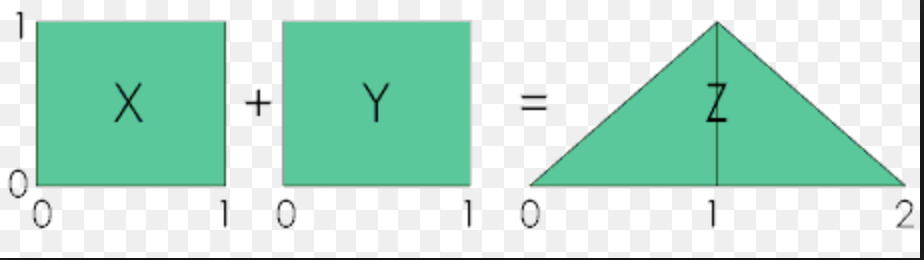
\includegraphics[scale = 0.8]{conv_u2.png}
\caption{The convolution of two uniform distributions $U[0,1]$.}
\end{figure}

This is actually why the distribution of dice rolls has a peak at $7$ and decreases in either direction, because it is the convolution of two uniform distributions (namely $U[1,6]$). 

In the discrete case, this is just 
\[ \PP(Z=k) = \sum_m \PP(X=m)\PP(Y=k-m).\] 

\subsection{Moment Generating Functions (Transforms)}
Recall from calculus that the exponential function has the series expansion 
\[ e^{sX} = 1 + sX + \dfrac{s^2}{2!}X^2 + \dfrac{s^3}{3!}X^3 + \dots.\] 
We can let $X$ be a RV. Then we can take expectation of both sides and apply linearity of expectation to get 
\[ M_X(s) = \EE[e^{sX}] = 1 + s\EE[X] + \dfrac{s^2}{2!}\EE[X^2] + \dfrac{s^3}{3!}\EE[X^3] + \dots .\] 

We call $M_X(s)$ the \textbf{moment generating function}, or \textbf{transform}, of $X$, for the following reason. All of the moments, i.e. RVs of the form $X^k$, are on the right hand side, and we can sift out whichever moment we need with a cute trick. If we want $\EE[X]$, then we can differentiate both sides with respect to $s$ and set $s = 0$, killing all the terms but $\EE[X]$. In symbols, 
\[ \dfrac{d}{ds}[M_X(s)] = \EE[X] + s\EE[X^2] + \dfrac{s^2}{2!}\EE[X^3] + \dots \] 
If we wanted $\EE[X^2]$, we can just take another derivative to get 
\[ \dfrac{d^2}{ds^2}[M_X(s)] = \EE[X^2] + s\EE[X^3] + \dots\] 
and set $s = 0$. In general, if we take $n$ derivatives, we find 
\[ \dfrac{d^n}{ds^n}[M_X(s)] = \EE[X^n] + s\EE[X^{n+1}] + \dots \]
from which setting $s$ to $0$ gives us the $n$th moment. 

What are the advantages of MGFs? 
\begin{enumerate}
    \ii Much easier to find the \emph{moments} of $X$. 
    \ii Much easier to \emph{multiply} than \emph{convolve}
    \ii Great analytical tool for proving things (CLT).
\end{enumerate}

Here's some properties. 
\begin{theorem}
    The moment generating function $M_X(s)$ of a RV $X$ satisfies the following properties. 
    \begin{enumerate}[(1)]
        \ii $M_X(0) = 1$. 
        \ii For $Y = aX + b$, $M_Y(s) = e^{sb}M_X(as)$.
    \end{enumerate}
\end{theorem}
\begin{proof}
    Part (a) is obvious. (Hint: use the very deep fact that $1 + 0 = 1$.)

    For part (b), just do the math. You get 
    \begin{align*}
        M_Y(s) &= \EE[e^{sY}] 
               = \EE[e^{s(aX+b)}] 
               = e^{sb}\EE[e^{asX}] = e^{sb} M_X(as).
    \end{align*}
\end{proof}

Let's get our hands dirty and find the MGFs of some common distributions. 
\begin{example}[Exponential MGF]
    Suppose we have a RV $X\sim \Expo(\la)$ which has pdf $f_X(x) = \la e^{-\la x}$ for $x\geq 0$. Then 
    \[ \EE[e^{sX}] = \int_0^{\infty} e^{sx}f_X(x) dx = \la\int_0^{\infty} e^{-\la x} e^{sx} dx = \la \dfrac{e^{-(\la-s)x}}{-(\la-s)} \Big|^{\infty}_0 = \dfrac{\la}{\la-s}\] 
    where $s < \la$ must hold in order for the integral to converge. Using this we can get $\EE[X] = M_X'(0) = \dfrac{\la}{(\la-s)^2}\Big|_{s=0} = \dfrac{1}{\la}$, and $\EE[X^2] = M_X''(0) = \dfrac{2}{\la}.$ 
\end{example}

\begin{example}[Poisson MGF]
    Now lets do the same for the Poisson distribution. Let $X\sim \Poisson(\la)$, so that $\PP(X=k) = \dfrac{e^{-\la}\la^k}{k!}$ for $k\geq 0$. Then 
    \[ M_X(s) = \EE[e^{sX}] = \sum_{k = 0}^\infty e^{sk}\dfrac{e^{-\la}\la^k}{k!} = e^{-\la}\sum_{k=0}^\infty \dfrac{(\la e^s)^k}{k!} = e^{-\la+\la e^s}.\]
    From this we can calculate $M_X'(0) = \la$ and $M_X''(0) = \la^2+\la$. 
\end{example}

\begin{example}[Normal MGF]
    Finally lets try the same for the normal distribution. Let $X\sim \Nor(0,1)$ so that $f_X(x) = \dfrac{1}{\sqrt{2\pi}}e^{-x^2/2}$. Then 
    \[ M_X(s) = \EE[e^{sX}] = \int_{-\infty}^\infty\dfrac{1}{\sqrt{2\pi}}e^{-x^2/2}e^{sx}dx.\]
    Now we're going to do a little bit of magic. The inside of this integral is $\exp(-x^2/2 + sx)$ which is a quadratic in $x$, so we're going to \emph{complete the square}. Hence, we get 
    \[ \dfrac{1}{\sqrt{2\pi}} \int_{-\infty}^\infty  \exp\left(-\dfrac{x^2-2xs+s^2}{2}\right) e^{s^2/2}dx = e^{s^2/2} \left[ \dfrac{1}{\sqrt{2\pi}} \int_{-\infty}^\infty e^{-(x-s)^2/2}dx\right].\]
    But the bracketed term is precisely our pdf integrated over its domain, which we already know to be 1. Hence, $M_X(s) = e^{s^2/2}$. This is super important, so know it. 

    If $Y\sim \Nor(\mu, \sigma^2)$, then $M_Y(s) = e^{s\mu}M_X(\sigma s)$, so $M_Y(s) = e^{s\mu}e^{\sigma^2s^2/2}$ is the MGF for general normal distributions. 
    
    It is left as an exercise to verifty that $M_X'(0) = 0$ and $M_X''(0) = 1$. 
\end{example}

\subsection{Inversions of transforms} 
Turns out $M_X(s)$ contains all of the info in $f_X(x)$ (under the mild condition that the moments are finite). This is known as the bilateral Laplace transform of $f_X(x)$. We can do inversions of these transforms using ``pattern matching,'' which is really just educating guessing lol. 

\begin{example}
    Suppose we have an MGF of $M_X(s) = \dfrac{1}{2}e^{-3s} + \dfrac{1}{4}e^{200s} + \dfrac{1}{4}e^s$. Recall that in the discrete case, transforms are a sum of terms of the form $e^{sx}$, so by comparing with the general formula 
  
    \[ M_X(s) = \sum_x e^{sx} p_X(x), \]

    we can recover our pdf as 
    \[ P(X = k) = \begin{cases}  
                    1/2 \quad \text{ when } k = -3 \\ 
                    1/4 \quad \text{ when } k = 200 \\ 
                    1/4 \quad \text{ when } k = 1 
            \end{cases} \] 
\end{example}

Here's the capstone on why we care so much about MGFs: we don't have to work with convolutions if we use them! Suppose we have $Z = X+Y$, where $X,Y$ are independent RVs. Then 
\[ M_Z(s) = \EE[e^{s(X+Y)}] = \EE[e^{sX}e^{sY}] = \EE[e^{sX}]\EE[e^{sY}],\]
avoiding any use of convolutions whatsoever! In summary, the MGF of the sum of two RVs is the product of their MGFs.

A quick application before we close out the day. Suppose $X\sim\Nor(\mu_X, \sigma_X^2)$ and $Y\sim\Nor(\mu_Y, \mu_Y^2)$. Then 
\[ M_Z(s) = M_X(s)M_Y(s) = \exp\left( \left(\dfrac{\sigma_X^2+\sigma_Y^2}{2}\right)s^2 + (\mu_X + \mu_Y)s \right) = MGF(\Nor(\mu_X+\mu_Y, \sigma_X^2+\sigma_Y^2)).\] 

\newpage
\section{Thursday, February 14th}
Happy Valentine's day to all the non-CS majors out there. As for the rest of you... 

\subsection{Moment Generating Functions (Review)}
The moment generating function of a random variable $X$ is $M_X(s) = \EE[e^{sx}]$, named as such because we can recover all of the moments $\EE[X^n]$ by taking derivatives. A quick result of this is that 
\[ \EE\left[\exp\left(s\sum_{i=1}^n X_i\right)\right] = \prod_{i=1}^n \EE[e^{sX_i}].\]

\subsection{Law of Total Variance}
 
\begin{theorem}[Total Variance]
    For random variables $X$ and $Y$, 
    \[ \Var(X) = \Var(\EE[X|Y]) + \EE[\Var(X|Y)].\] 
\end{theorem}
\begin{proof}
We expand intelligently; 
\begin{align*}
    \Var(X) &= \EE[(X-\EE[X])^2] \\ 
            &= \EE[(X - \EE[X|Y] + \EE[X|Y] - \EE[X])^2] \\ 
            &= \EE[(X-\EE[X|Y])^2] + 2\EE[(X-\EE[X|Y])(\EE[X|Y]-\EE[X])] + \EE[(\EE[X|Y] - \EE[X])^2] 
\end{align*}
where the last step was performed by grouping the first two terms and the last two terms and expanding. ``It is left as an exercise to show the middle term goes to 0,'' so we will focus on what we get from the remaining two terms. 

We will make use of the following fact. 

\begin{theorem}[Iterated Expectation]
    For random variables $X$ and $Y$, 
    \[ \EE[{\color{red}X}] = \EE[\EE[{\color{red}X} | {\color{blue}Y}]].\] 
\end{theorem}

You can think of this as conditional expectation; we condition on $Y$ and find the expectation on the inside, and then ``sum out'' over all values of $Y$ by taking an expectation on the outside. Hence, we can rewrite 
\begin{align*}
    \EE[{\color{red}(X-\EE[X|Y])^2}] &= \EE[\EE[{\color{red}(X-\EE[X|Y])^2} | {\color{blue}Y}]] = \Var(\EE[X|Y]) \\
\EE[(\EE[X|Y] - \EE[{\color{red}X}])^2] &= \EE[(\EE[X|Y] - \EE[\EE[{\color{red}X}|{\color{blue}Y}]])^2] = \EE[\Var(X|Y)]
\end{align*}
from which our result follows 
\end{proof}

Here's an application as a quick reality check. \footnote{Thanks to Efe for the Piazza explanation.}

\begin{example}
    A chocolate store receives $B\sim \Bin(n,p)$ types of chocolate. When you go to the store, for each type of chocolate in the store, you toss an independent coin which has a probability $q$ of success. In summary, the amount of chocolate you buy is $C = \sum_{i = 1}^B \one_i$ where $\one_i$ is a Bernoulli RV with probability $q$. 

    We can compute the variance of $C$ using the law of total variance, which tells us that 
    \[ \Var(C) = \Var(\EE[C|B]) + \EE[\Var(C|B)].\] 
    
    First, notice that $C|B$ is a RV according to $\Bin(B, q)$; there are $B$ chocolates, and we have a probability $q$ of buying each one. Then $\EE[C|B]$ is $Bq$ by linearity of expectation, so 
    \[ \Var(Bq) = q^2\Var(B) = q^2np(1-p).\] 
    Also, $\Var(C|B)$ is $Bq(1-q)$, so 
    \[ \EE[Bq(1-q)] = q(1-q)\EE[B] = npq(1-q).\] 
    Putting it all together gives 
    \[ \Var(C) = npq^2(1-p) + npq(1-q) = npq(q-pq + 1-q) = npq(1-pq),\]
    which is precisely the variance of $\Bin(B, pq)$! This shouldn't be surprising, since we expected that the total number of things compounds in this way. 
\end{example}

\subsection{Tail Bounds: Markov and Chebyshev}
This consists of a lot of CS 70 material (Markov's, Chebyshev's), but also some new bounds (namely the Chernoff bound). 

\begin{theorem}[Markov's Inequality]
    For a nonnegative random variable $X$, 
    \[ \PP(X \geq t) \leq \dfrac{\EE[X]}{t}\] 
    for all $t > 0$. 
\end{theorem}

This is important because tail bounds help us bound rare things that are away from the expectation. Think of a statistician who wants to bound the probability of errors in his/her data
% Insert picture of markov's on a normal distribution
\begin{proof}
    We condition on values of $X$, so 
    \begin{align*}
        \EE[X] &= \EE[X | X \leq t] \PP(X\leq t) + \EE[X | X \geq t]\PP(X\geq t) \\ 
               &\geq 0 + t \PP(X\geq t)
    \end{align*}
    where we can lower bound by $0$ since $X$ is nonnegative and we can lowerbound $\EE[X|X\geq t]$ by $t$ since we're conditioning on $X\geq t$. 
\end{proof}

The proof in our book uses coupling, which is creating a new random variable which is $0$ when $X\leq t$ and exactly $t$ when $X\geq t$, which leads to a similar proof as shown here. 

Let's try applying Markov's inequality to an exponential distribution $X\sim \Expo(\la)$. We have $\PP(X\geq t) = e^{-\la t}$ by the CDF, while Markov's inequality gives a bound of $\frac{1}{\la t}$, which is much looser. This might lead one to think that Markov's inequality is weak, but if all you know about a distribution is its mean, Markov's inequality is actually \emph{tight}! For a fixed $t$, there are distributions for which equality holds.

Of course, if you know more information you can obtain a better bound. Namely, 

\begin{theorem}[Chebyshev]
    For a random variable $X$, 
    \[ \PP(|X-\EE[X]| \geq t) \leq \dfrac{\Var(X)}{t^2}\] 
    for $t>0$.
    \label{thm:chebyshev}
\end{theorem}
\begin{proof}
    Using the very deep fact that $|a| > b \implies a^2 > b^2$, we find that 
    \[ \PP(|X-\EE[X]|\geq t) = \PP((X-\EE[X])^2 \geq t^2) \leq \dfrac{\EE[(X-\EE[X])^2]}{t^2} = \dfrac{\Var(X)}{t^2}\]
    where we can use Markov's inequality since $(X-\EE[X])^2$ is nonnegative. 
\end{proof}

\begin{example}
    Let $X\sim \Bin(n,p)$. By Markov, 
    \[ \PP(|X-\EE[X]|\geq t) \leq \dfrac{\EE[|X -\EE[X]|]}{t} \leq \dfrac{\EE[|X|+|\EE[X]|]}{t} = \dfrac{2\EE[X]}{t} = \dfrac{2np}{t}\] 
    where we used the triangle inequality to deduce that $|X-\EE[X]| \leq |X| + \EE[X]$ (triangle inequality is $|a+b| < |a| + |b|$), and $\EE[\EE[X]] = \EE[X]$ since expectation of a constant is a constant. 
    
    If we use Chebyshev, we get a bound of 
    \[ \PP(|X-\EE[X]|\geq t) \leq \dfrac{\Var(x)}{t^2} = \dfrac{np(1-p)}{t^2}\] 
    which is a factor of $t$ tighter than Markov. 
\end{example}

\subsection{Chernoff Bounds}

Before we go into Chernoff bounds, let's try to motivate them and see why they are interesting. Let's try bounding the probability $\PP(X\geq t)$ by the moments. By Markov, we have 
\[ \PP(f(X) \geq f(t)) \leq \dfrac{\EE[f(X)]}{f(t)}\] 
for $f(X) \geq 0$ and for all $f(t) > 0$. Hence, we can see that 
\[ \PP(X \geq t) \leq \dfrac{\EE[f(X)]}{f(t)}\] 
provided that $\PP(X\geq t) \leq \PP(f(X) \geq f(t))$; this can be achieved if $f$ is monotonically increasing, but this is merely sufficient, not necessary. 

Using this derived bound, we can bound probabilities by moments of our random variable by taking $f(t) = t^n$ to get  
    \[ \PP(X \geq t) \leq \dfrac{\EE[X^n]}{t^n}\] 
for $X\geq 0$, which is pretty good. The Chernoff bound is similar, offering us a bound in terms of the moments. 

\begin{theorem}[Chernoff Bound]
    For a random variable $X$, 
    \[ \PP(X\geq t) \leq \dfrac{\EE[e^{\la X}]}{e^{\la t}}\]
    for all $t$ and $\la > 0$.
\end{theorem}
\begin{proof}
    This should be second nature at this point. . Since $\la > 0$, 
    \[ \PP(X\geq t) = \PP(\la X \geq \la t) = \PP(e^{\la X} \geq e^{\la t}) \leq \dfrac{\EE[e^{\la X}]}{e^{\la t}}.\] 
\end{proof}

Important question of the day: why do we even need a $\la$ at all? 

Answer: Like the French revolution, it gives you freedom! (over how sharp of a bound you get). One thinks of it as a knob that you can adjust to give you a better (or worse) bound. Note that higher $\la$ isn't always better. 

Another note is that Chernoff bounds aren't always the best; if you have a Chernoff bound with a fixed $\la$, I can always come up with a better moment bound. 

\begin{example}
    Let's apply the Chernoff bound to normal random variables. We find that 
\[ \PP(X\geq t) \leq \dfrac{\EE[e^{-\la X}]}{e^{\la t}} = \dfrac{e^{-\la^2\si^2/2}}{e^{\la t}}\] 
for $X\sim \Nor(0, \si^2)$. We want to pick the $\la$ that minimizes this, so we'll take logs and then differentiatie, because 
\[ \arg\min_\la \dfrac{e^{-\la^2\si^2/2}}{e^{\la t}} = \arg\min_\la \dfrac{\la^2\si^2}{2} - \la t.\] 
    Differentiating this gives a solution $\la  = t/\si^2$, which gives a bound of $\PP(X\geq t) \leq e^{-t^2/2\si^2}$, which is literally as tight as possible since it's our CDF. Magic. 
\end{example}

\newpage
\section{Thursday, February 21st}
\subsection{Announcements}
HW 5 due next Wednesday. Reading is B\&T 5.2-5.6, Walrand 2.1-2.3. Apparently Chapter 2 is quite difficult to read, so proceed with caution. %Today is a lot of concentration variables.

\subsection{Weak and Strong Law of Large Numbers (Modes of Convergence)}
The idea of the weak law of large numbers is to look at the behavior of say coin flips in the long run. There's two questions we can start off our discussion with: how many heads (mean) will we get, and how variable are our results (variance)? 

We can describe it formally as such. We perform an experiment $n$ times independently and note 
\[ M_n = \dfrac{1}{n}\sum_{i=1}^n X_i \quad (X_i's \text{ i.i.d. })\] 
where $X_i$ has mean $\mu$ and variance $\sigma^2$. Then 
\[ \EE[M_n] = \EE\left[\dfrac{1}{n}\sum_{i=1}^n X_i\right] = \dfrac{1}{n} \EE[X_1]\cdot n = \EE[X_1] = \mu,\] 
and 
\[ \Var(M_n) = \dfrac{1}{n^2}\sum_{i = 1}^n \Var(X_i) = \dfrac{\si^2}{n}\] 
since the $X_i$ are i.i.d. If we take $n\to\infty$ to look at the long term behavior, $\EE[M_n] = \mu$ and $\Var(M_n) = 0$. 

This is cool and all, but wouldn't it be dope if we also knew the \emph{rate} at which the variance decreased to 0? We can do this by using Chebyshev (Theorem~\ref{thm:chebyshev}) to do a tail bound:
    \[ \PP(|M_n-\mu| > \epsilon) \leq \dfrac{\si^2}{n\epsilon^2},\]
     and just like that we've derived the weak law of large numbers. 
\begin{theorem}[Weak LLN]
    Suppose $X_1, X_2, \dots, X_n$ are i.i.d. RVs with mean $\mu$. Then for any $\epsilon > 0$, 
\[ \PP\left(\left|\dfrac{X_1+X_2+\dots + X_n}{n}-\mu\right| \geq \epsilon\right) \to 0 \]
    as $n\to\infty$. 
\end{theorem}

What does the Weak LLN really mean? In one way, it means that $\lim_{n\to\infty}\PP(|M_n-\mu|\geq \epsilon) = 0$. Now recall delta-epsilon limits from calculus: for any $\epsilon, \delta > 0$, there exists $n(\epsilon, \delta)$ (meaning $n$ is a function of $\epsilon,\delta$), large enough such that 
    \[ \PP(|M_n-\mu|\geq\epsilon) \leq \delta\] 
for $n> n(\epsilon, \delta).$ We can think of these variables as representing the following: 
\begin{align*}
    \epsilon &: \text{ ``accuracy level'' or error } \\ 
    \delta &: \text{ confidence level } \\ 
    n(\epsilon, \delta) &: \text{ threshold for a given accuracy/confidence } 
\end{align*}

Motivated by our above findings, we make an important definition: 

\begin{definition}
    We say a sequence of random variables $(M_n)_{n=1}^\infty = M_1, M_2, \dots$ \textbf{converges in probability} if for any $\epsilon > 0$, $\PP(|M_n-\mu| \geq \epsilon)\to 0$ as $n\to\infty$, and denote it as $M_n\cinprob \mu$. 
\end{definition}

This gives us a notion of convergence for random variables/distributions, much like convergence of functions from Calculus.\footnote{Remember $\delta - \epsilon$ limits? yea those disgusting things.}

\begin{example}
    Suppose $X_1, X_2, \dots, X_n \sim U[-1, 1]$ are i.i.d., and $Y_n = \frac{X_n}{n}$. Then to find the density, we first find that 
    \[ Y_n \leq y \implies X_n \leq ny,\]
    so 
    \[ F_{Y_n}(y) = F_X(ny) \implies f_{Y_n}(y) = n f_X(ny). \] 
    %%%%%%%%%%% INSERT GRAPH %%%%%%%%%%%%%%
    If we plot $f_{Y_n}(y)$, it would be a rectangle with endpoints at $y = -1/n$ and $y = 1/n$ with height $n/2$ since $f_{Y_n}(y) = n/2$ for all $y$ in its domain. Then $\PP(|Y_n| \geq \epsilon) = 0$ if $n > \frac{1}{\epsilon}$, which is what it means to converge in probability. 
\end{example}

\begin{example}
    Let $Y_n = \min(X_1, X_2, \dots, X_n)$ where $X_i$'s are i.i.d. in $U[0,1]$. Then 
    \[ \PP(|Y_n - 0| \geq \epsilon) = \PP(X_1\geq \epsilon, X_2\geq \epsilon, \dots, X_n > \epsilon) = (1-\epsilon)^n \xrightarrow[n\to\infty]{\PP} 0 .\] 
    In other words, the probability that the minimum is greater than any $\epsilon$ you pick in the long run is $0$, which makes sense. 
\end{example}

\begin{example}
    Suppose time is in discrete units\footnote{``Bold move.'' - Phil} $(1, 2, \dots )$ and $Y_n = 1$ if there is an arrival at time $n$, $Y_n = 0$ otherwise. Define $I_k = \{2^k, 2^k+1, \dots, 2^{k+1}-1\}$, so that every next interval is twice as large as the next one. 
    %%%%%%%%%%%%%%%%%%%%%%%%%%%%%%%%%%%%%%%%%%%
    %
    %-----------------------------------------
    % 1 2 3 4 5 6 7 8 9 ...  15 16 
    %I0  I1 |--I2--| |---I3---|
    %
    %%%%%%%%%%%%%%%%%%%%%%%%%%%%%%%%%%%%%%%%%%%
    Suppose there is exactly $1$ arrival in each interval (equally likely). Then 
    \begin{align*}
        \PP(Y_1 = 1) &= 1 \\ 
        \PP(Y_2 = 1) = \PP(Y_3 = 1) &= \dfrac{1}{2} \\ 
                                    &\dots \\ 
        \PP(Y_n = 1) &= \dfrac{1}{2^k} \text{ if } n \in I_k.
    \end{align*}
    
    So $\lim_{n\to\infty}\PP(Y_n = 1) = \lim_{k\to\infty}\frac{1}{2^k} = 0$, meaning that $\PP(Y_n=1)$ converges to $0$ in probability. 
    
    This should be confusing however! Given any finite $n$, there are certain to be an infinite number of arrivals after $n$. Hence, we know for a \emph{fact} that $\PP(Y_n=1)$ will be nonzero infinitely often. 
    
    This example demonstrates the weakness of the weak LLN, and tells us that perhaps there are stronger notions of convergence than just convergence in probability. 
\end{example}

Before I state Strong LLN, I will first state what this stronger notion of convergence is. 

\begin{definition}
    Let $(M_n)_{n\geq 1}$ be a sequence of random variables. Then we say that $M_n$ converges \textbf{almost surely} to $\mu$ if 
    \[ \PP\left(\lim_{n\to\infty} M_n = \mu\right) = 1\] 
    and denote it by $M_n\asure \mu$. 
\end{definition}

\begin{theorem}[Strong LLN]
    Let $(X_n)_{n\geq 1}$ be a sequence of i.i.d. RV's with mean $\mu$. Then, 
    \[ \dfrac{1}{n}\sum_{i=1}^n X_i \to \mu \] 
    as $n\to\infty$ with probability $1$. In other words, if we let $M_n = \frac{1}{n}\sum X_i$, then $M_n\asure \mu$. 
\end{theorem}

\begin{proof}
    Walrand Chapter 2, but only for the brave. 
\end{proof}

Let's illustrate the difference between the Weak and Strong LLN with an example of rolling 6-sided die. The Strong LLN states that \emph{every} realization converges to $\mu$. So if we were to draw a plot of all different realizations, the Strong LLN states that all of them tend towards the line $X = \mu$. 

\begin{figure}[!htb]
\centering
    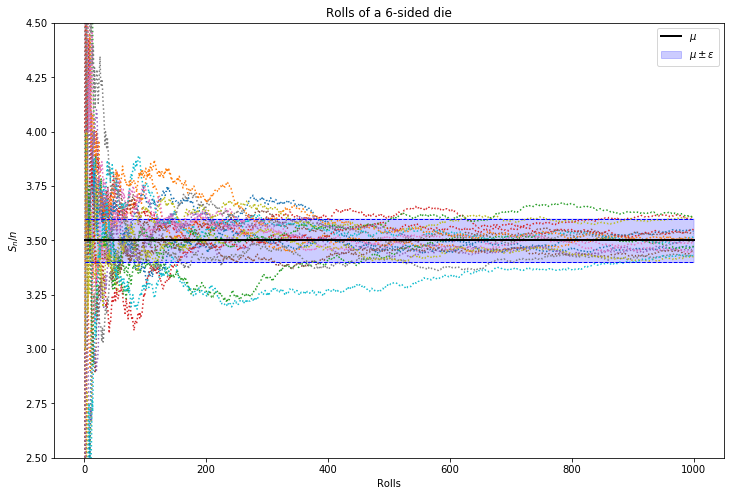
\includegraphics[scale=0.61]{LLN.png}
    \caption{The weak LLN bounds the long-run values with the blue bounding box $X \in [\mu-\epsilon, \mu + \epsilon]$, while strong LLN asserts all values become the black line, $X = \mu$.}
\end{figure}

On the other hand, the Weak LLN only places a bounding box of width $2\epsilon$ around our mean, and says that the probability of any realizations outside this box is 0 in the long run. It doesn't say anything about occurences within the box, which is why our wacky example from above technically converges in probability. Hence, all we are guaranteed is that the \emph{fraction} of realizations outside $\mu\pm \epsilon$ for all $\epsilon, \delta > 0$ converges to $0$. 

\subsection{The Central Limit Theorem}

\begin{question}
    What happens to $S_n = \sum_{i = 1}^n X_i = X_1 + X_2 + \dots + X_n$ as $n\to\infty$?
\end{question}
\begin{proof}[Answer]
    You always end up with a normal distribution. Try it out for $X_i \sim U[0,1]$ or $X_i \sim \Exp(1)$ if you don't believe me. 
\end{proof}

    If we look at the variance and mean of $S_n\to \infty$ as $n\to\infty$, then we find that $\EE[S_n] = n\mu$ and $\Var(S_n) = n\si^2$. Hence we should normalize by defining 
\[ Z_n = \dfrac{S_n - n\mu}{\sqrt{n}\si}.\] 
You can check that this now has 0 mean and variance 1. As before, we might expect that this new random variable is normal if the $X_i$ are uniform or exponential, so that $Z_n$ is just a standard normal distribution. Amazingly, this holds in general, which is what the CLT states. 

\begin{theorem}[Central Limit Theorem]
    Suppose $S_n = \sum_{i=1}^n X_i$ where the $X_i$ are i.i.d. RVs with mean $\mu$ and variance $\si^2$, and define $Z_n$ as above. Then, (amazingly), 
    \[ \lim_{n\to\infty} \PP(Z_n\leq x) = \Phi(x) \] 
    where $\Phi(x)$ is the c.d.f of the standard normal distribution $\Nor(0, 1)$. 
\end{theorem}

For large enough $n$, $Z_n\sim\Nor(0,1)$ in distribution, i.e. 
\begin{align*}
    S_n &\xrightarrow[n\to\infty]{d} \Nor(n\mu, n\si^2) \\
    Z_n &\xrightarrow[n\to\infty]{d} \Nor(0, 1) 
\end{align*}

where $\xrightarrow[n\to\infty]{d}$ is convergence in distribution, which we will not go into detail about. There are two implications. 
\begin{enumerate}
    \ii The distribution of $S_n$ and $Z_n$ ``wipe out'' all the information except for $\mu$ and $\si^2$. 
    \ii If there are a large number of small independent factors, the \emph{aggregate} of these factors will be normally distributed, which is just noise. 
\end{enumerate}

We end the day by outlining the proof of CLT. 
\begin{proof}[Proof of CLT]
    If $Y\sim \Nor(0,1)$, $M_Y(s) = \EE[e^{sY}] = e^{s^2/2}$. Then suppose $X_1, X_2, \dots, X_n$ are i.i.d. with mean $0$ and variance $1$ (WLOG). Let $M_X(s)$ be the MGF of each $X_i$, and let 
    \[ Z = \dfrac{X_1 + X_2 + \dots + X_n}{\sqrt{n}} \implies \EE[Z] = 0, \Var(Z) = 1.\] 
    Then 
    \[ M_Z(s) = \EE[e^{sZ}] = \EE[\exp(\frac{s}{\sqrt{n}}(X_1 + X_2 + \dots + X_n))].\] 
    We can finish the proof then by decomposing $M_Z(s)$ and using Taylor expansion. The rest of the proof will be discussed next week. 
\end{proof}

\newpage
\section{Tuesday, February 26th}
HW 5 is due tomorrow, and the readings are Walrand Ch 1, 2.4, 13.3, B\&T 6.1-6.4. 

\subsection{Wrapping up CLT}
From last lecture, suppose we have $S_n = \sum_{i=1}^n X_i$ where $X_i$ are i.i.d. with mean $\mu$ and variance $\si^2$. Then if let 
\[ Z_n = \dfrac{S_n - n\mu}{\sqrt{n}},\]
as $n\to\infty$, $Z_n$ has mean $0$ and variance $1$, giving us information about the long-term behavior of $S_n$. The Central Limit Theorem tells us more precisely that $\PP(Z_n\leq x) = \Phi(x)$ for every $x$. Let's prove CLT. 

\begin{proof}[Proof of CLT]
Let $X_1, X_2, \dots, X_n$ be i.i.d. with mean $0$ and variance $1$ and let $M_X(s)$ be the MGF of each of the $X_i$'s. Note that by definition, 
\[ Z = \dfrac{X_1 + X_2 + \dots + X_n}{\sqrt{n}} \implies \EE[Z] = 0, \Var(Z) = 1.\] 

Our goal is to be able to find the MGF of $Z$ as well. If we expand, we will get 
\begin{align*}
    M_Z(s) = \EE[e^{sZ}] &= \EE\left[e^{s\frac{1}{\sqrt{n}}(X_1 + X_2 + \dots + X_n)}\right] \\ 
                         &= \EE\left[e^{\frac{sX_1}{\sqrt{n}}}\right] \EE\left[e^{\frac{sX_2}{\sqrt{n}}}\right]\dots  \EE\left[e^{\frac{sX_n}{\sqrt{n}}}\right] \\ 
                         &= \EE\left[e^{\frac{sX_i}{\sqrt{n}}}\right]^n = \left[M_X\left(\frac{s}{\sqrt{n}}\right)\right]^n 
\end{align*}

Now recall Taylor's theorem: any infinitely differentiable function can be written as $f(x) = f(a) + f'(a)(x-a) + \dots + f^{(n)}(a)(x-a)^n + \dots$ (the \emph{Taylor} Series). So, 
\begin{align*}
    M_X(s) &= M_X(0) + M_X'(0)s + M_X''(0)\dfrac{s^2}{2!} + M_X'''(0)\dfrac{s^3}{3!}+\dots\\ 
           &= 1 + \EE[X]s + \EE[X^2]\dfrac{s^2}{2} + \EE[X^3]\dfrac{s^3}{6}\dots \\ 
           &= 1 + \dfrac{1}{2}s^2 + \dfrac{s^3}{6}\EE[X^3] 
\end{align*}

where we used our earlier facts that $\EE[X] = 0$ and $\EE[X^2] = \Var(X)+\EE[X]^2 = 1$. Plugging this into our MGF for $Z$ gives 
\[ M_Z(s) = \left[M_X\left(\frac{s}{\sqrt{n}}\right)\right]^n = \left[1 + \dfrac{s^2}{2n} + \dfrac{s^3}{6n^{3/2}}\EE[X^3] + \dots \right]^n\]  
\[ \implies \lim_{n\to\infty} M_Z(s) = \lim_{n\to\infty} \left[ 1 + \dfrac{s^2}{2n} + \dfrac{s^3}{6n^{3/2}}\EE[X^3] + \dots \right]^n.\] 

This looks really similar to our classic limit of the form $\lim_{n\to\infty}(1+\frac{x}{n})^n = e^x$, but its got these higher order terms that we'd ideally like to ignore. Turns out that those terms actually don't matter; the only ones we care about are the first two. We write this as $o(\frac{1}{n})$ (little $o$ notation) to show that in the limit these terms disappear, so 
\[ \lim_{n\to\infty} M_Z(s) = \lim_{n\to\infty} \left[1+\dfrac{s^2/2}{n} + o\left(\dfrac{1}{n}\right)\right]^n = e^{s^2/2} = M_Y(s)\] 
completing our proof. 
\end{proof}

Here's an application of CLT to testing light bulbs. 
\begin{example}
    Light bulbs have i.i.d $\Expo(\la)$ lifetimes. We want to make sure that $\frac{1}{\la} > 1$. Say we measure the average lifetimes $A_n$ of $n = 100$ bulbs and find $A_{100} = 1.2$. Then $A_n = \frac{1}{n}\sum_{i=1}^n S_i$, so 
    \begin{align*}
        \EE[A_n] &= \frac{1}{\la} \\ 
        \Var(A_n) &= \frac{1}{n^2}\cdot n \cdot \frac{1}{\la^2} = \frac{1}{n\la^2}. 
    \end{align*}
    \begin{question}
        What is the confidence that we have $\frac{1}{\la} > 1$? 
    \end{question}
    Let $Z_n = \dfrac{A_n - \frac{1}{\la}}{\frac{1}{\la\sqrt{n}}}$, so that $Z_n$ has $0$ mean and variance $1$. Then by CLT, $Z_n\sim \Nor(0,1)$. Taking $n = 100$ gives 
    \[ Z_{100}  = \dfrac{A_{100} - \frac{1}{\la}}{\frac{1}{10\la}} = 10(1.2\la -1) = 12\la - 10.\] 
    So to find our probability, we simply calculate 
    \[ \PP(\la < 1) = \PP(12\la - 10 < 2) = \PP(\Nor(0,1) < 2) = 97.5\%\] 
    Note this approximation is an asymptotic estimation and not a bound, but a damn good one at that. 
\end{example}

\subsection{Information Theory}
This entire field was born with Claude Shannon's 1948 paper \emph{A mathematical theory of communication}, which was actually rejected from the publishing journal Shannon sent it to for not being rigorous enough. The reviewer of the paper remarked 30 years later that, ``One of my biggest regrets was rejecting that paper.'' 


\begin{figure}[!ht]
    \centering
    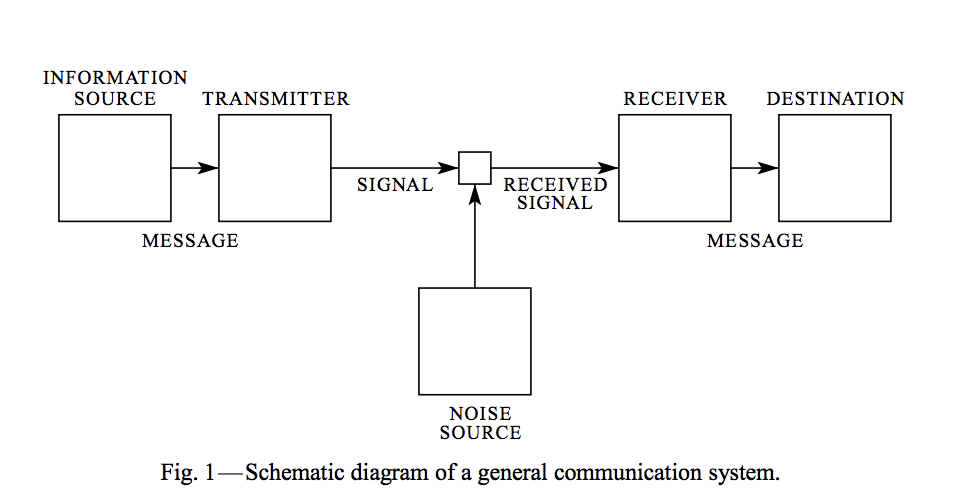
\includegraphics[scale=0.8]{shannon_paper_fig.png}
\caption{Shannon's proposed communication framework (Shannon 1948).}
\end{figure}

\begin{theorem}[Separation]
    There is no loss of optimality in separating source-coding (compression) from channel coding (reliable communication). 
\end{theorem}

\begin{example}[Source Coding]
    Let $X\sim\{0,1\}$ with $\PP(X=1) = p$, and let $X^{(n)} = \{010\dots\}$ be an $n$-length $\Ber(p)$ source. Suppose we have a file of length 10,000. and it was $\Ber(p)$ i.i.d. What is the compression limit?  

    The entropy $H(X)$ is 
    \[ H(X) = -\sum_{x\in\{0,1\}}p(x) \log p(x) = -p\log p - (1-p)\log(1-p) = h(p).\] 
    If we plot $h(p)$, we can see a parabola like shape with a maximum of $1$ at $p = 0.5$, so we can't compress it at all. If $p = 0.11$, then $h(p) = 0.5$ between symbols, so a 10,000 length file has a 5,000 length compression limit. 
\end{example}

If one is interested in more Information Theory, look into taking EE 229A. 

\subsection{Asymptotic Equipartition Property}
If I have an $n$-length $\Ber(p)$ sequence, we will have $np$ heads and $n(1-p)$ tails. Then AEP says that out of the $2^n$ total sequences, the number of sequences that I can expect to see, $\binom{n}{np}$, is approximately $2^{n h(p)}$ (using Stirling's apprx.), so each sequence appears with probability $2^{-n h(p)}$. 

We also talked about Binary Erasure Channels and their capacities. See the next lecture for more info. 

\newpage
\section{Thursday, February 28th}
HW 6 is released, due next Wednesday. Reading is Walrand Chapter 1, 13.3 and B\&T Chapters 7.1-7.4, plus the notes on BECs. 

\subsection{Capacity of the BEC}
Recall that a \textbf{Binary Erasure Channel} is a model where a transmitter sends a bit, either 0 or 1, through a channel, and the receiver either receives the bit or is notified that the message was erased. Here is an illustration. 

\begin{figure}[!htb]
\centering
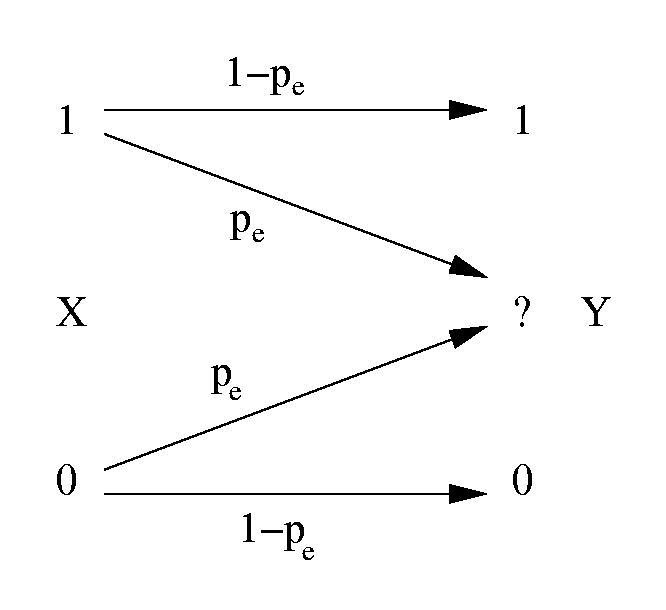
\includegraphics[scale=0.2]{BEC.png}
\caption{In a BEC, our transmissions are erased with probability $p_e$. Source: Wikipedia}
\end{figure}

The goal of today is to find the \emph{capacity} of the BEC$(p)$ channel. Capacity is the maximum rate of reliable communication, which we can define as 
\[ \text{ Rate } = \dfrac{ \text{\# of bits reliably sent}}{\text{\# of channel uses}} = \dfrac{L(n)}{n} \text{ bits/ch use}.\]

We also make the following definitions (which can be seen in the diagram): 

\[ f_n(\cdot) \text{ is the encoding function that maps } \{0,1\}^L\to\{0,1\}^n \] 
\[ g_n(\cdot) \text{ is the decoding function that maps } \{0,1, *\}^n\to\{0,1\}^L \] 

We can let $P_e^{(n)} = \max_{m=\{0,1\}^L} \PP(m\not= \hat{m})$ denote the probability of error. Let me explain why this makes sense. We take the max to get the ``worst case'' error, and we take $m = \{0,1\}^L$ as an approximation of sending many messages. Of course, the probability is precisely the event of an error, when our sent message is different from the decoded message.

Finally, let $R = L/n \text{ bits/channel use}$. We say that rate $R$ is \emph{achievable} for the channel if for every $n$, there exists encoding and decoding functions such that $P_e^{(n)} \xrightarrow[n\to\infty]{} 0$ (which exact mode of convergence is t.b.d.). The largest achievable rate $R$ is called the \textbf{capacity} of the channel, denoted $C_{\BEC{p}}$. 

Now the stage is set for us to state Shannon's theorem. 
\begin{theorem}[Shannon 1948]
    $C_{\BEC{p}} = 1-p$ bits per channel use. 
\end{theorem}

There are two statements hidden within this theorem. The capacity of the BEC is at most $1-p$, and that this maximum is also attainable. 

\begin{proof}
    We first show that the capacity cannot exceed $1-p$. Assume we have a friendly genie who relays instantaneously to the sender (TX) whenever the received symbol is a $*$. Then the best rate is to resend whichever symbols are erased. Hence, the time for a bit to get through the channel is approximately $\Geo(1-p)$, so the expected time it takes a bit to get through is $1/(1-p)$ channels per bit. Hence, $C \leq 1-p$ bits per channel use. 

    Now we do the forward direction to show this maximum is attainable. We'll show that $R = 1-p-\epsilon$ for all $\epsilon > 0$ is achievable. Shannon's insight was to leverage the Strong LLN. By Strong LLN, the probability of channel erases exactly $np$ symbols is $1$. In other words, as $n\to\infty$, $\PP(np\text{ bits erased})\to 1$. 

    Next we populate a lookup table of size $2^L$ by $n$ with i.i.d. $\Ber(1/2)$ entries. Call this table a \emph{codebook} $\mathcal{C}$, and allow it to be shared between the sender and the receiver before hand. 

\begin{figure}[!ht]
\[ \begin{array}{C|C|C|C|C|C}
    & 1 & 2 & 3 & \dots & $n$ \\
\hline
1 & 1 & 1 & 0 & \dots & 1 \\
2 & 0 & 1 & 1 & \dots & 0 \\
3 & 1 & 0 & 1 & \dots & 0 \\
$\vdots$ & $\vdots$ & $\vdots$ & $\vdots$ & $\ddots$ & $\vdots$ \\
$2^L$ & 1 & 0 & 0 & \dots & 1 \\
\end{array} \]
\caption{An example of a codebook $\mathcal{C}$.}
\end{figure}


    Suppose we transmit a message in the $i$th row of $\mathcal{C}$. On average, by SLLN, there are $np$ bits that are erased. WLOG assume they are at the end of the message. The receiver will drop the last $np$ columns of the codebook to obtain a truncated codebook $\mathcal{C}'$. Then he will follow these rules for decoding: 
    \begin{enumerate}
        \ii If $c_j'$ is the \emph{only} entry in $\mathcal{C}'$ matching $Y^{(n(1-p))}$ ($Y^n$ without the last $np$ bits), then decode $\hat{m} = j$. 
        \ii Else, declare ERROR. 
    \end{enumerate}
    If this sounds like a really dumb idea you're not wrong. But it turns out this is just enough for us to attain the maximum. To see this, we need to calculate the probability of an error.  
\begin{align*}
    \PP(\text{error}) = \PP(c'_i\text{ is not unique}) 
    &= \PP\left(\bigcup_{i\not= j} \{c_i' = c_j'\}\right) \\ 
    &= \sum_{i\not= j} 2^{-n(1-p)} < 2^L 2^{-n(1-p)}
\end{align*}
by the union bound. Hence, $P_e \leq 2^{n(R-(1-p))}$. In order for $P_e \xrightarrow[n\to\infty]{} 0$, we need $R-(1-p) < 0$, or $R < 1-p$. So we just make $R = 1-p-\epsilon$ so that $P_e \leq 2^{-n\epsilon} \xrightarrow[n\to\infty]{} 0$ for all $\epsilon > 0$. 
\end{proof}

Here's a quick engineering example with some numbers. 
\begin{example}
    Suppose we take $n = 10,000$, $p = 1/2$ and $\epsilon = 0.01$. Then 
    \[ C_{\BEC{\frac{1}{2}}} = \dfrac{1}{2} \text{ bits/ch. use } \implies C = 5000\text{ bits.}\] 
    So we set our $R$ to $1-\frac{1}{2} - 0.01 = 0.49$ which means $L = 4900$ bits. Hence $P_e \leq 2^{-n\epsilon} = 2^{-100} \approx 0$. This means that we can can send $4900$ with basically no errors. Neat. 
\end{example}

\subsection{Markov Chains}

We will often want to study stochastic processes $X = \{X_t\}_{t\in T}$, which are a collection of RVs, where the index $t$ often refers to a representation of time. $X$ models the evolution of a sequence of RVs as a function of time. Some examples are stock prices, your wealth, customers, etc. 

In general, to characterize the behavior of $X: (X_1, X_2, \dots, X_n)^\infty$, we would need the joint pdf of $X_1, X_2, \dots, X_n$. This is a \emph{bad idea}, since it will very quickly grow too large for any reasonable computation. Hence we impose some structure on the process and get a markov chain. 

\begin{definition}
    Let $\mathcal{X}$ be a finite set (called the state space) with random variables $X_i$ drawn from it. Then if 
    \[ \PP(X_n = x_n | X_{n-1} = x_{n-1}, \dots, X_1 = x_1) = \PP(X_n = x_n | X_{n-1} = x_{n-1}),\] 
    we call $X_n$ a \textbf{Markov Chain}.
\end{definition}
The above property is called the ``amnesia'' or Markov property, since your state today only depends on your state yesterday and so on. 
Based on the Markov Chain, you can also come up with its transition matrix, which is just a matrix that encodes the Markov property, $\PP(X_n | X_{n-1})$. 


\newpage
\section{Tuesday, March 5th}
I couldn't go this day, but all we convered was CS 70 level Markov Chain. Note 21 would be a good review here. 

\newpage
\section{Thursday, March 7th}
HW 7 is due next Wednesday, Lab 4 due tomorrow. Reading is Walrand Chapters 1, 2.4-2.6, 13.3 and B\&T Sections 7.1-7.4. 

These notes are still under construction; there's some pictures I need to add, edits I need to make but I have important deadlines these two weeks :(.

\subsection{Discrete Time Markov Chains}
Recall that we have two important notions regarding DTMCs: 
\begin{itemize}
    \ii If a finite Markov Chain is \emph{irreducible}, it has a unique invariant distribution $\pi^*$. 
    \ii If a Markov Chain is also \emph{aperiodic}, $\lim_{n\to\infty} \pi_n^* = \pi^*$. 
\end{itemize}

\begin{example}
    Flip a fair coin repeatedly until you get 3 successive heads. What is the expected number of coin flips to 3 consecutive heads?
\end{example}

    We can do this by defining a Markov Chain where the states are the number of successive heads, since the only information that matters for us is the number of heads in a row. 

    \begin{figure}[!ht]
\begin{center}
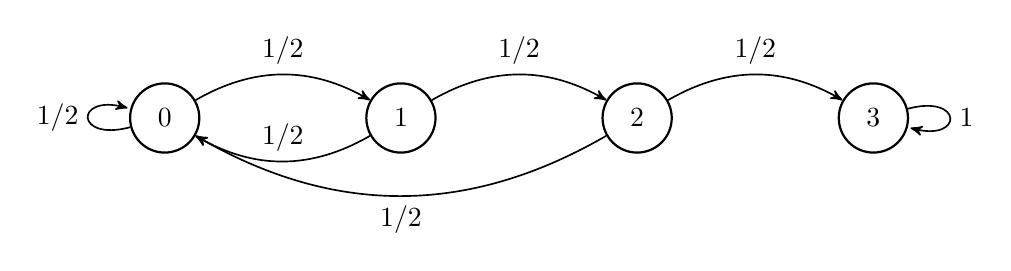
\begin{tikzpicture}[->, >=stealth', auto, semithick, node distance=3cm]
\tikzstyle{every state}=[fill=white,draw=black,thick,text=black,scale=1]
\node[state]    (A)               {$0$};
\node[state]    (B)[right of=A]   {$1$};
\node[state]    (C)[right of=B]   {$2$};
\node[state]    (D)[right of=C]   {$3$};
\path
(A) edge[loop left]     node{$1/2$}         (A)
    edge[bend left, above]    node{$1/2$}      (B)
(B) edge[bend left, above]    node{$1/2$}           (C)
    edge[bend left, above]     node{$1/2$}           (A)
(C) edge[bend left, above]    node{$1/2$}           (D)
    edge[bend left, below]     node{$1/2$}           (A)
(D) edge[loop right]     node{$1$}           (D);
\end{tikzpicture}
\end{center}
\caption{Casting the problem with a Markov Chain}
\end{figure}

We are looking for $T_3 = \min( n\geq 0 , X_n = 3)$. Define $\beta(i) = \EE[T_3 | X_0 = i]$ for $i = 0, 1, 2, 3$, so that $\beta(i)$ is the expected number of steps it takes to reach state $3$ from state $i$. Our First-Step Equations (FSEs) are 
\begin{align*} 
    \beta(0) &= 1 + \frac{1}{2}\beta(1) + \frac{1}{2}\beta(0) \\ 
    \beta(1) &= 1 + \frac{1}{2}\beta(2) + \frac{1}{2}\beta(0) \\ 
    \beta(2) &= 1 + \frac{1}{2}\beta(3) + \frac{1}{2}\beta(1) \\ 
    \beta(3) &= 0.
\end{align*}

Solving gives us $\beta(3) = 0$, $\beta(2) = 8$, $\beta(1) = 12$, and $\beta(0) = 14$ which is our desired answer. 

\begin{example}
    A clumsy drunk monkey climbs a ladder. He goes up one step with probability $p = 0.8$, otherwise he slips to the ground. What is the average time taken to go to the $n$th rung (say $n=10$)?
\end{example}

The states here should be the number of rungs climbed so far. Clearly we are interested in hitting time of the state $n$ from the state $0$. Here's the Markov Chain for this situation: 

\begin{figure}[!ht]
\begin{center}
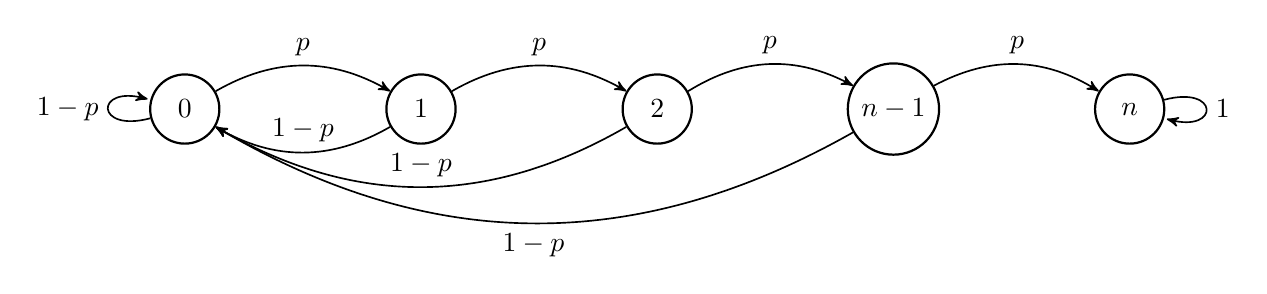
\begin{tikzpicture}[->, >=stealth', auto, semithick, node distance=3cm]
\tikzstyle{every state}=[fill=white,draw=black,thick,text=black,scale=1]
\node[state]    (A)               {$0$};
\node[state]    (B)[right of=A]   {$1$};
\node[state]    (C)[right of=B]   {$2$};
\node[state]    (D)[right of=C]   {$n-1$};
\node[state]    (E)[right of=D]   {$n$};
\path
(A) edge[loop left]     node{$1-p$}         (A)
    edge[bend left, above]    node{$p$}      (B)
(B) edge[bend left, above]    node{$p$}           (C)
    edge[bend left, above]     node{$1-p$}           (A)
(C) edge[bend left, above]    node{$p$}           (D)
    edge[bend left, above]     node{$1-p$}           (A)
(D) edge[bend left, above]     node{$p$}           (E)
    edge[bend left, below]     node{$1-p$}           (A)
(E) edge[loop right]     node{$1$}           (E); 
\end{tikzpicture}
\end{center}
\caption{The drunk monkey Markov Chain}
\end{figure}

We can calculate our First Step Equations to be 
\begin{align*}
    \beta_m &= 1 + p\beta_{m+1} + (1-p)\beta_0 \text{ for } m = 0, 1, \dots, n-1 \\ 
    \beta_n &= 0 
\end{align*}
It is \emph{obvious} to see from here that the solution is $\beta_0 = \dfrac{1-p^n}{p^n - p^{n+1}}$. If $p = 0.8$ and $n = 10$ as we desire, then $\beta_0 = 41.5$, which is a very long time for the poor monkey. 

\subsection{General Hitting Times}
Moving to generality, we can state hitting times of not just singular states, but sets of states, in Markov Chains. Suppose we have a Markov Chain $\mathcal{X}$ on a state space $\mathcal{S}$ with transition matrix $P$. Then for some subset $A\subseteq \mathcal{S}$, the \textbf{hitting time} $T_A$ of that subset is defined as 
\[ T_A = \min\left\{n\geq 0 | x_n \in A\right\}. \] 

We can define First Step Equations as usual in the following way. Let $\beta(i) = \EE[T_A | X_0 = i]$. Then, 
\[ \beta(i) = \begin{cases} 
        1 + \sum_{j} P(i,j)\beta(j) \quad &\text{ if } i\not\in A \\ 
        0 \quad &\text{ if } i\in A.
    \end{cases} 
\]

Here's another applciation of the same approach. I want to find the probability of hitting a set $A$ before hitting a set $B$, where $A$ and $B$ are disjoint sets (why is this important?). Define $\alpha(i) = \PP(T_A < T_B | X_0 = i)$ as the probability we hit $A$ before $B$ when we start at $i$, where 
\[ T_A = \min_{n\geq 0} \{ X_n \in A \}\] 
is the hitting time of set $A$. Then our FSEs in this case are 
\[ \alpha(i) = \begin{cases} 
        0 \quad &\text{ if } i\in B \\
        1 \quad &\text{ if } i\in A \\
        \sum_{j} P(i,j)\alpha(j) \quad &\text{ if } i\not\in A\cup B.
    \end{cases} 
\]

A classic application of this setup is the Gambler's Ruin, but we won't discuss it for the sake of time. 

\subsection{Classification of General DTMCs}
\begin{definition}
    A state $i$ is said to be \textbf{transient} if given that we start at state $i$, there is a nonzero probability that we never return to state $i$. Otherwise the state is \textbf{recurrent}, i.e. we will return to state $i$ with probability $1$. 
\end{definition}

There's a good illustration of recurrent and transient states on page 350 of B\&T. They're pretty easy to understand lol. 


\begin{figure}[!ht]
    \centering
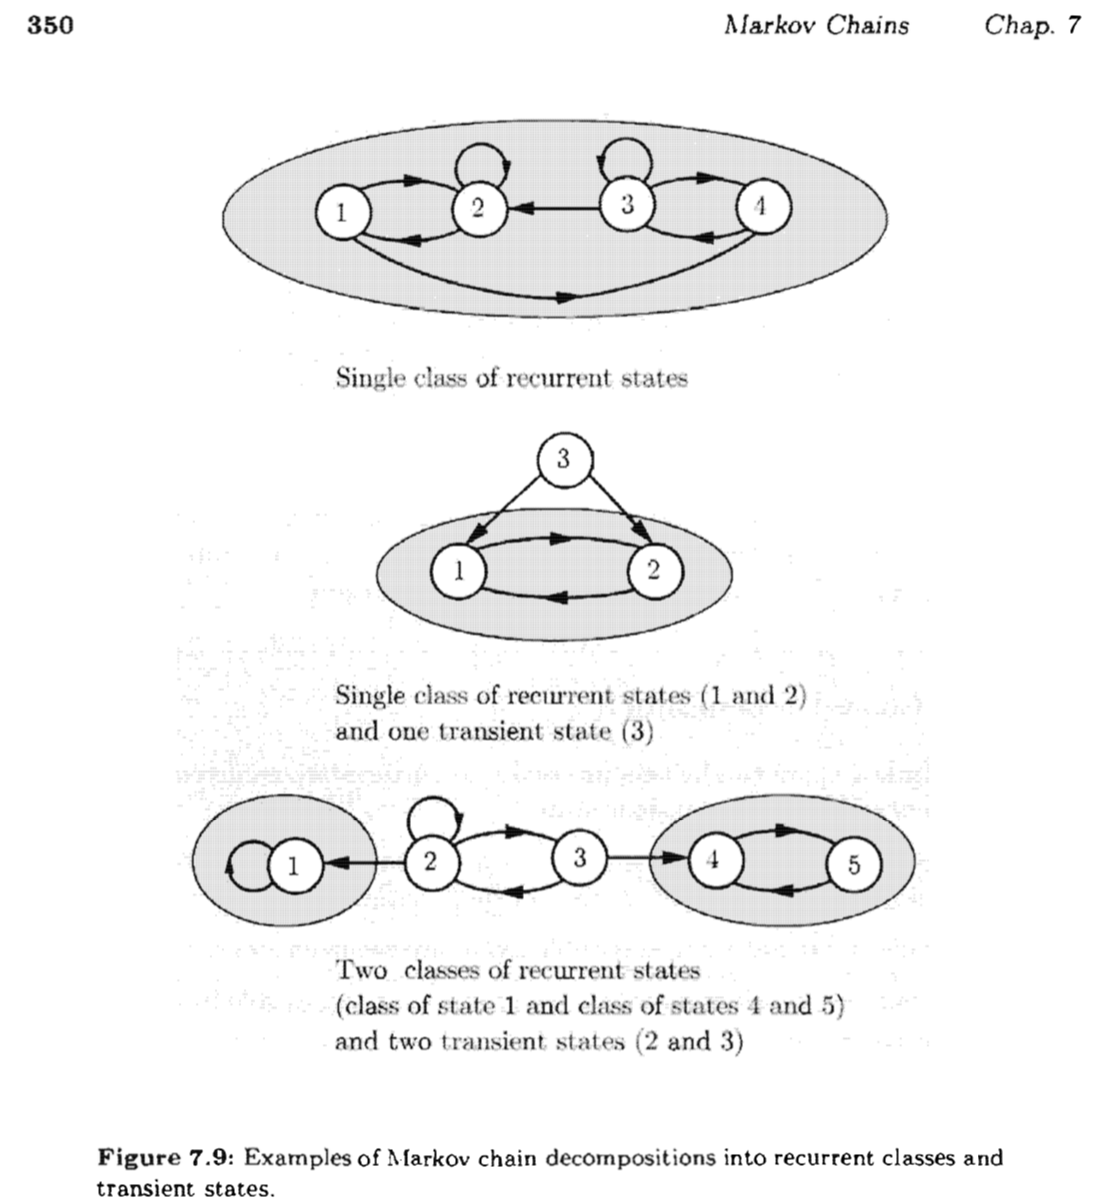
\includegraphics[scale = 0.7]{recurrent_transient.png}
\caption{Page 350 of Bertsekas and Tsitsiklis.}
\end{figure}

Futhermore, if an irreducible Markov Chain is recurrent, then 
\[ \text{if }
    \begin{cases}
        \EE[T_i | X_0 = i] < \infty \quad &\text{ positive recurrent}  \\
        \EE[T_i | X_0 = i] = \infty \quad &\text{ null recurrent}  
    \end{cases}
\]
The idea is that there are two different classes of recurrent. Recurrence implies that you eventually return to your state; positive recurrence just means you return within some finite time, whereas null recurrence means you return to that state ``in theory'', but realistically you really don't. 

\iffalse
\begin{figure}[!ht]
\begin{center}
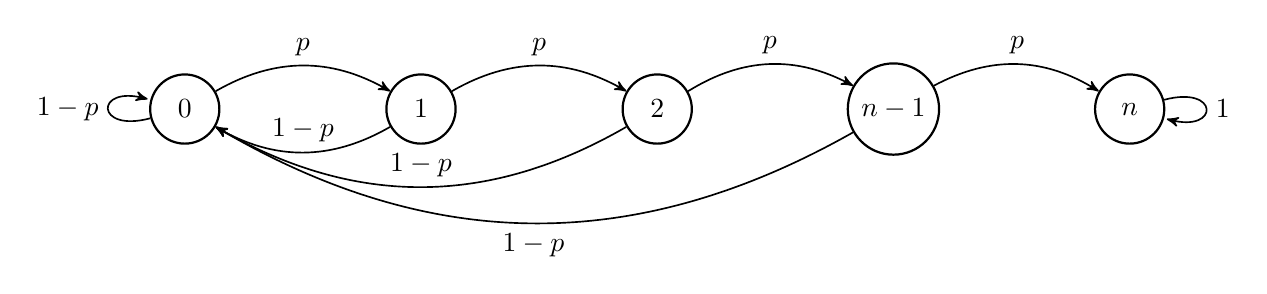
\begin{tikzpicture}[->, >=stealth', auto, semithick, node distance=3cm]
\tikzstyle{every state}=[fill=white,draw=black,thick,text=black,scale=1]
\node[state]    (A)               {$0$};
\node[state]    (B)[right of=A]   {$1$};
\node[state]    (C)[right of=B]   {$2$};
\node[state]    (D)[right of=C]   {$n-1$};
\node[state]    (E)[right of=D]   {$n$};
\path
(A) edge[loop left]     node{$1-p$}         (A)
    edge[bend left, above]    node{$p$}      (B)
(B) edge[bend left, above]    node{$p$}           (C)
    edge[bend left, above]     node{$1-p$}           (A)
(C) edge[bend left, above]    node{$p$}           (D)
    edge[bend left, above]     node{$1-p$}           (A)
(D) edge[bend left, above]     node{$p$}           (E)
    edge[bend left, below]     node{$1-p$}           (A)
(E) edge[loop right]     node{$1$}           (E); 
\end{tikzpicture}
\end{center}
\caption{Casting the problem with a Markov Chain}
\end{figure}
\fi

There's a cool example of a markov chain called the \emph{Gambler's Ruin} problem which is either transient, positive recurrent, or null-recurrent. I'll add it in once I create time to do so. 

Now we have a Big theorem. 
\begin{theorem}[Walrand 13.2]
    Suppose we have a finite Markov Chain. Then we can classify when a Markov Chain is transient, positive recurrent, or null-recurrent. To be added. 
\end{theorem}

We end on a cute example of a null recurrent Markov Chain. 
\begin{figure}[!ht]
\begin{center}
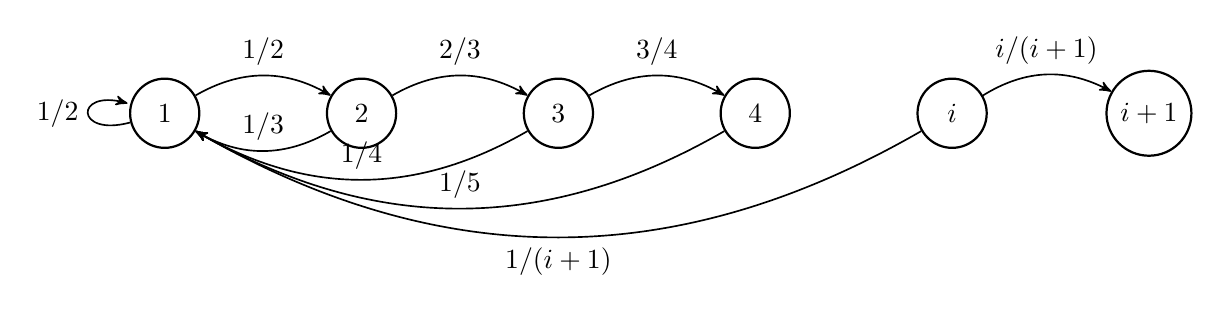
\begin{tikzpicture}[->, >=stealth', auto, semithick, node distance=2.5cm]
\tikzstyle{every state}=[fill=white,draw=black,thick,text=black,scale=1]
\node[state]    (A)               {$1$};
\node[state]    (B)[right of=A]   {$2$};
\node[state]    (C)[right of=B]   {$3$};
\node[state]    (D)[right of=C]   {$4$};
\node[state]    (E)[right of=D]   {$i$};
\node[state]    (F)[right of=E]   {$i+1$};
\path
(A) edge[loop left]     node{$1/2$}         (A)
    edge[bend left, above]    node{$1/2$}      (B)
(B) edge[bend left, above]    node{$2/3$}           (C)
    edge[bend left, above]     node{$1/3$}           (A)
(C) edge[bend left, above]    node{$3/4$}           (D)
    edge[bend left, above]     node{$1/4$}           (A)
(D) edge[bend left, above]     node{$1/5$}           (A)
(E) edge[bend left, above]     node{$i/(i+1)$}           (F)
    edge[bend left, below]     node{$1/(i+1)$}           (A); 
\end{tikzpicture}
\end{center}
\caption{Null Recurrence}
\end{figure}

If we calculate the hitting time of $T_1$, we find that 
\[ \EE[T_1 | X_0 = 1] = \dfrac{1}{2} \cdot 1 + \dfrac{1}{2}\cdot\dfrac{1}{2}\cdot 2 + \dfrac{1}{2}\cdot\dfrac{2}{3}\cdot\dfrac{3}{4}\cdot 3 + \dots \]

TBF. 

\newpage
\section{Tuesday, March 12}
HW 7 is due tomorrow, Lab 5 due Friday. Reading for DTMC's is Walrand Ch. 1, 2.4-2.6, and 13.3; B\%T 7.1-7.4. Reading for Poisson Processes is Walrand 13.4 and B\&T 6.1-6.3. 

\subsection{DTMC's: Recap of Recurrence, Transience}
This was a recap of the gambler's ruin like example. Didn't catch it, but I'll edit it in once I get time (spring break?).

\subsection{Reversibility Markov Chains}
Assume we have an irreducible and positive recurrent Markov Chain started at its unique invariant distribution $\pi$. Suppose for every $n$, $(X_0, X_1, \dots, X_n)$ has the same joint pmf as the time-reversed chain $(X_n, X_{n-1}, \dots, X_0)$. Then we call the chain \emph{reversible}. 

\begin{fact}
    Reversible or not, if we start a MC at its invariant distribution $\pi$, the time-reversed sequence is a Markov Chain.  
\end{fact}
\begin{proof}
    We have that 
    \begin{align*}
        \PP(X_k = i | X_{k+1} = j, X_{k+2} = i_{k+2}, \dots, X_n = i_n) &= \dfrac{\PP(X_k = i, X_{k+1} = j, \dots, X_n = i_n)}{\PP(X_{k+1} = j, X_{k+2} = i_{k+2}, \dots, X_n = i_n)}  \\
        &= \dfrac{\pi(i) P_{i,j}P_{j, i_{k+2}} \dots P_{i_{n-1},i_n}}{\pi(j) P_{j, i_{k+2} } \dots P_{i_{n-1}, i_n}} \\ 
        &= \dfrac{\pi(i) P_{i,j}}{\pi(j)}
    \end{align*}
    Hence, $\tilde{P}_{j,i} = \dfrac{\pi(i) P_{i,j}}{\pi(j)}$, which only depends on $i,j$, so the sequence is a Markov Chain. 
\end{proof}

From this proof, we can see that for reversibility, we need 
\[ \tilde{P}_{ji}(\text{reverse chain})= P_{ij}(\text{forward chain}).\]
This is satisfied when 
    \[ \pi(j) \tilde{P}_{j,i} = \pi(i) P_{i,j}\]
    for all $i,j\in \mathcal{X}$ in a reversible Markov Chain. We call these the \textbf{detailed balance equations}, but Ramchandran likes to call them Local Balance Equations. 

\begin{theorem}
    If a Markov Chain is reversible, then it has an invariant distribution $\pi$. 
\end{theorem}

Recall that if a Markov Chain has an invariant distribution $\pi$, $\pi = \pi P$. We call this the \emph{Global Balance Equation}, as opposed to the Local Balance Equations from above. 

\begin{proof}
    Suppose we have some distribution of states $\pi$. Then 
    \[ \sum_i \pi(i) P_{i,j} = \sum_i \pi(j) \tilde{P}_{j,i} = \pi(j) \sum_{i} \tilde{P}_{j,i} = \pi(j).\] 
    Hence for every $j$, the local balance equations imply a global balance equation,  so $\pi = \pi P$, and so our Markov Chain has an invariant distribution. 
\end{proof}

We can employ reversibility to solve for transience in the earlier example. Here's another quick application. 

\begin{figure}[!ht]
\begin{center}
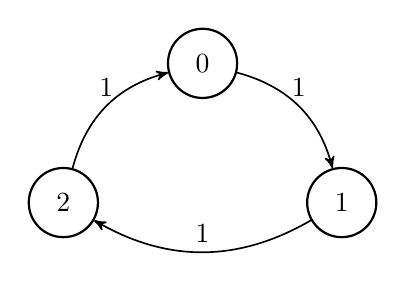
\begin{tikzpicture}[->, >=stealth', auto, semithick, node distance=2.5cm]
\tikzstyle{every state}=[fill=white,draw=black,thick,text=black,scale=1]
\node[state]    (A)               {$0$};
\node[state]    (B)[below right of=A]   {$1$};
\node[state]    (C)[below left of=A]   {$2$};
\path
(A) edge[bend left, above]    node{$1$}      (B)
(B) edge[bend left, above]    node{$1$}    (C)
(C) edge[bend left, above]    node{$1$}   (A); 
\end{tikzpicture}
\end{center}
\caption{Is this chain reversible?}
\end{figure}

Is this chain reversible? If we list the possible states going forwards and backwards, they are  

\begin{align*}
    \text{Forwards: } & 012012\dots \\ 
    \text{Backwards: } & 210210\dots 
\end{align*}

but we can never get from 2 to 1 in this chain. Hence, it is not reversible. Another way to see this is that by the local balance equations, 
\[ \pi_0(1) = \pi_1(0) = 0,\] 
so $\pi_0 = 0$. Similarly, $\pi_1 = 0$ and $\pi_2 = 0$ which is a contradiction, since they must add up to 1. 

There's some other cool ways to determine if a Markov Chain is reversible. One of them is \href{https://en.wikipedia.org/wiki/Kolmogorov%27s_criterion}{Kolmogorov's criterion}, which gives a necessary and sufficient condition based on only the transition probability. Out of scope though. 

\subsection{Introduction to Poisson Processes}
Possion Processes are continuous versions of the ``coin-flipping'' or Bernoulli processes, where ``arrival'' times are continuous. Some motivation is that it's a good model for arrivals of packets at a router, photons hitting a photon detector, etc. 

One way to define Poisson Processes, which is the way Walrand follows and so will we, is to have $S_1, S_2, \dots, S_n$ which are i.i.d. $\Expo(\la)$ ($\la >0$) RVs, and define $T_i$'s as the CT arrival times. Then we can count arrivals as 
\[ N_t = \begin{cases} 
        \max_{n\geq 1} \{ n | T_n \leq t \} &\text{ if }t\geq 0 \\ 
        0 &\text{ if } t < T 
    \end{cases} 
\] 

\newpage 
\section{Thursday, March 14} 
Happy $\pi$ day everyone. HW 8 is out, due next Wednesday, Lab 5 is due on Friday (tomorrow), and the Reading is on Poisson Processes, Walrand 13.4 and B\&T 6.1-6.3. 

\subsection{Poisson Processes}
We can define Poisson processes by their arrival times, but also their interarrival times $S_i$, where $S_i \sim \Expo(\la_i)$. Then $T_n = \sum_{i = 1}^n S_i$ is our Poisson Process. 

Let's do a quick review of Exponential RVs first. Recall that the density of the exponential distribution is $f_{S_i}(t) = \la e^{-\la t}$. Then the CDF is just 
\[ F_{S_i}(t) = \PP(S_i \leq t) = \begin{cases}
        1 - e^{-\la t} &\text{ if } t\geq 0 \\ 
        0 &\text{ else }
    \end{cases} 
\] 
We also have that $\EE[S_i] = 1/\la$ and $\Var(S_i) = 1/\la^2$, and of course the memoryless property, which says that 
\[ \PP(S_i > t + s | S_i > s) = \PP(S_i > t),\] 
i.e. the probability of an arrival is independent of how long we've waited. 

Also, 
\[ \PP(S_i \leq t + \epsilon | S_i > t) = \la\epsilon + o(\epsilon),\] 
where $o(\epsilon)$ are the higher order terms, i.e. terms of the form $\epsilon^2, \epsilon^3$, etc. Formally, $\lim_{e\to 0} \frac{o(\epsilon)}{\epsilon} = 0$. 

Why? Well by memoryless, 
\[ \PP(S_i > t + \epsilon | S_i > t) = \PP(S_i > \epsilon) = e^{-\la \epsilon} = 1 - \la\epsilon + o(\epsilon)\] 
by a Taylor Series expansion. Then subtracting from $1$ gives us our result above. 

Now divide up an interval into $\epsilon$ long chunks. For each interval, let's ask the question of how many arrivals we will have in such an interval. Using our previous derivations, we find that 
\begin{align*}
    \PP(\text{no arrivals in this interval}) &= 1- \la\epsilon + o(\epsilon) \\ 
    \PP(\text{1 arrival in an }\epsilon \text{ interval}) &= \la\epsilon + o(\epsilon) \\ 
    \PP(\text{2 or more arrivals in the interval}) &= 1 - (1-\la\epsilon + \la\epsilon + o(\epsilon)) = o(\epsilon)
\end{align*}
Hence as $\epsilon \to 0$, the probability of there being more than 1 arrival in any interval quickly goes to $0$. So we can treat the Poisson Process also as arrivals within $\epsilon$ wide intervals, which is how the Bertsekas textbook defines PPs. From here, one can show that the interarrival times follow exponential distributions, but this is pretty clunky, so we defined them the other way around like Walrand does. We'll see later the motivation for doing so this way. 

Here's a theorem that shouldn't be surprising. 
\begin{theorem}
    Poisson processes are memoryless. 
\end{theorem}

One can think of Poisson processes as inheriting this memoryless property from exponential distributions. But what does it mean for a process to be memoryless? We know what it means for RVs to be memoryless; turns out the equivalent notion is similar. In pictures, if $N_t$ is a $\PoisP(\la)$, then so is $N_{t+s} - N_t$. 

Here's some implications. For starters, $\PoisP(\la)$ has \emph{independent} and \emph{stationary} increments. For any $0\leq t_1 \leq t_2 \leq \dots$, $\{N_{t+s} - N_t\}$ are independent and distribution depends only on $t_{n+1} - t_n$. 

\begin{proof}[Proof with words]
    A $\PoisP{\la}$ has inter-arrival times that are independent $\Expo(\la)$ RVs. So, for $t > T_3$ in the picture, it is obvious that the inter-arrival times are $\Expo(\la)$ by constraint. The only possible issue is with the \emph{first} arrival (i.e. $s < T_3 - t$). But, by the memoryless property of the $\Expo(\la)$ RV, the first inter-arrival distribution is also $\Expo(\la)$. 
\end{proof}

You're probably also wondering by this point, why the hell are these called Poisson Processes? Literally everything about these processes has been exponential, so where does the Poisson come in? Here's why. 

\begin{theorem}[Walrand 13.7]
    If $\mathcal{N} = \{N_t, t\geq 0\}$ is a $\PoisP(\la)$, then $N_t$, the \# of arrivals in $(0,t)$, has a $\Poisson(\la t)$ distribution, i.e. 
    \[ \PP(N_t = k) = e^{-\la t} \dfrac{(\la t)^k}{k!} \] 
        for $k \geq 0$.
\end{theorem}

There's two proofs, one which uses a clever symmetry argument and another with differential equations. We're going to sketch the former thankfully. Bertsekas actually assumes this property of Poisson Processes and goes backwards to show inter-arrival times are exponential. Two equivalent ways of motivating Poisson Processes. 
\begin{proof}
    If our goal is to find the distribution of $N_t$, then we need a density for the number of arrivals in $(0,t)$. This means we will first find the joint density of $T_1, T_2, \dots, T_k, T_{k+1}, \dots$. This is equivalent to 
    \[ \PP(T_1 \in \{t_1, t_1 + dt_1\}, T_2\in\{t_2, t_2 + dt_2\}, \dots, T_k\in\{t_k, t_k + dt_k\}, T_{k+1} > t).\] 
    We'd like to convert these to $S_i$'s however, because they're exponentials and easy to work with. So doing so gives 
    \[ \PP(S_1 \in \{0, t + dt_1\}, S_2 \in\{ t_2 - t_1, t_2-t_1+dt_2\}, \dots, S_k\in\{t_k-t_{k-1}, t_k-t_{k-1}+dt_k\}, S_{k+1} > t-t_k).\] 
    We can approximate the probability of $S_i \in t_i + dt_i$ as a rectangular region whose area is $f_{S_i}(t_i)\cdot dt_i = \la e^{-\la t_i} dt_i$, so this probability reduces to 
\begin{align*}
    (\la e^{-\la t_1} dt_1)(\la e^{-\la (t_2-t_1)}dt_2)(\la e^{-\la (t_3 - t_2)}dt_3)\dots (\la e^{-\la (t_k-t_{k-1})}dt_k) (e^{-\la(t-t_k)}) \\ 
    = \la^k e^{-\la t} dt_1 dt_2 \dots dt_k 
\end{align*}
by cancellation (!! sick !!). Hence, 
\[ \boxed{f_{T_1, T_2, \dots, T_k}(t_1, t_2, \dots, t_k) = \la^k e^{-\la t}}.\] 

Now notice that $f$ is \emph{uniform} over the support of $(T_1, T_2, \dots, T_k)$. Hence, 
\[ N_t(k) = \int_{t_1}\int_{t_2}\dots \int_{t_k} f_{T_1, T_2, \dots, T_k}(t_1, t_2, \dots, t_k) dt_1dt_2\dots dt_k.\] 
The inside is independent of $t_1, \dots, t_k$, so 
\[ N_t(k) = \la^k e^{-\la t} \int_0^t \int_0^t \dots \int_0^t dt_1dt_2\dots dt_k\] 
\textbf{subject} to the constraint that the arrivals happen in order, i.e. $S: t_1 < t_2 < \dots < t_k$. 

Without any constraints, $Vol(S) = t^k$. But this accounts for \emph{all} permutations of $(t_1, \dots, t_k)$. By symmetry, all permutations have the \emph{same} volume though! There are $k!$ different permutations, of which $1$ is actually legal. Hence the volume we actually care about is $\frac{1}{k!} t^k$. Combining all together, we get that 
\[ N_t(k) = \la^k e^{-\la t} \left(\dfrac{1}{k!}t^k\right) = e^{-\la t} \dfrac{(\la t)^k}{k!}\] 
as desired. 
\end{proof}
Cleeeeean. 

\subsection{Splitting and Merging of Poisson Processes}
If we have have two independent PPs $\PoisP(\la_1)$ and $\PoisP(\la_2)$, we can \textbf{merge} them to be a $\PoisP(\la_1 + \la_2)$. 

Likewise, if we have a $\PoisP(\la)$, then it can split into two Poisson Processes $\PoisP(\la p)$ and $\PoisP(\la(1-p))$ where $p$ is the probability of choosing an interval to split or not. That's basically all there is to splitting and merging, so let's do some examples. 

\begin{example}[Fishing]
    Bob catches fish according to a Poisson Process with rate $\la = 0.6$ fish/hr. If he catches at least one fish in the first $2$ hours, he quits (after two hours). Else, he continues till he has caught the first fish. 
\end{example}
    
\begin{question}
    What is $\PP(\text{Bob fishes for}>\text{2 hours})$? 
\end{question}

    Answer: Happens only if he catches 0 fish in $[0,2]$ hours, which is $\PP(N(2) = 0) = e^{-\la 2} = e^{-1.2}$ by using the CDF. 

\begin{question}
    What is $\PP(\text{Bob fishes for time} t\in[2,5]\text{ hours})$? 
\end{question}

    Answer: Two events must occur: he must catch no fish in $[0,2]$, and also catch one fish in $[2,5]$. The first event has probability $e^{-1.2}$, while the second event has probability $1-e^{-1.8}$. By independence, our overall probability is $e^{-1.2}(1-e^{-1.2})$. 

\begin{question}
    What is $\PP(\text{Bob catch at least 2 fish})$? 
\end{question}

    Answer: Similar to the beginning of lecture. $1-e^{-1.2}-1.2e^{-1.2}$.  

\begin{question}
    What is $\EE[\text{fish caught by Bob}]$? 
\end{question}
    
    Answer: By Linearity of Expectation, 
    \[ \EE[\text{fish caught}] = \EE[\text{fish caught in} (0,2)] + \EE[\text{fish caught in} (2, \infty)] \] \[= 1/(\la t) + 1\cdot e^{-2\la} = 1.2 + e^{-1.2}.\] 

\newpage
\section{Tuesday, March 19th}
Readings on CTMC are Walrand 13.5 and B\&T, 7.5. 

\subsection{Poisson Processes Recap}
We did a lot of review of last week; the first new thing we did was the following example. 

\begin{example}
    Two light bulbs have burn out times distributed according to $\Expo(\la_a)$ and $\Expo(\la_b)$ respectively. What's the expected first burn out time of either light bulb? 
\end{example}

We can treat the burn out times as a Poisson Process, where each of the lightbulbs have  parameters $\la_a$ and $\la_b$. Then the expected first burn out (a.k.a. the $\min$ of the two random variables) is equivalent to the first arrival of the merged processes, which would be distributed according to $\Expo(\la_a+\la_b)$. 

\subsection{Erlang Distributions}

\subsection{Random Incidence Phenomenon}
 

\newpage
\section{Thursday, March 21st}

\subsection{Continuous Time Markov Chains}

\subsection{Balance Equations}

\subsection{Hitting Times}


\newpage
\section{Tuesday, April 2nd}
HW 9 is due tomorrow. We have a midterm next Tuesday, and there are review sessions on Saturday, April 6th from 1-3pm. Reading on Random Graphs is to be posted. 

\subsection{Wrap up CTMC's}
Here's an example of a continous time markov chain. 

\begin{figure}[!ht]
\begin{center}
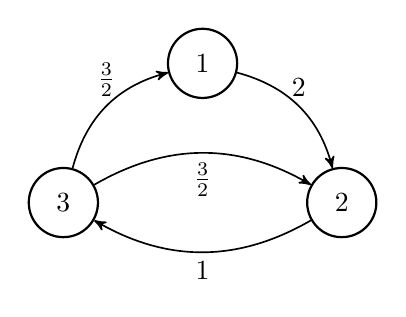
\begin{tikzpicture}[->, >=stealth', auto, semithick, node distance=2.5cm]
\tikzstyle{every state}=[fill=white,draw=black,thick,text=black,scale=1]
\node[state]    (A)               {$1$};
\node[state]    (B)[below right of=A]   {$2$};
\node[state]    (C)[below left of=A]   {$3$};
\path
(A) edge[bend left, above]    node{$2$}   (B)
(B) edge[bend left, below]    node{$1$}   (C)
(C) edge[bend left, above]    node{$\frac{3}{2}$}   (A) 
    edge[bend left, below]    node{$\frac{3}{2}$}   (B);
\end{tikzpicture}
\end{center}
\caption{A Continuous Time Markov Chain}
\end{figure}

Our transition matrix is just 
\[ Q = \bbm -2 & 2 & 0 \\ 0 & -1 & 1 \\ \frac{3}{2} & \frac{3}{2} & -3 \ebm\]

Then to find the stationary distribution, we just solve for the $\pi$ such that $\pi Q = 0$ and $\sum \pi_i = 1$. We get 
\[ \pi = \dfrac{1}{19} [3\quad 12\quad 4].\] 
 
But what if we wanted to calculate the amount of time we're spending to get from one state to another? It's clear what the transitions are since the rates are specified, but it's not so clear how we quantify time spent at each state. The out-going rates at state $1$, 2, is slower than the out-going rate at state $3$, 3, which would make it unfair to compare their times naively.

The solution then is to scale our times according to the ``fastest'' clock, which would be state 3's clock in this case. Suppose you want to find $\pi$ based on equating it to a DTMC. Then we can construct the following discretized markov chain. 

\begin{figure}[!ht]
\begin{center}
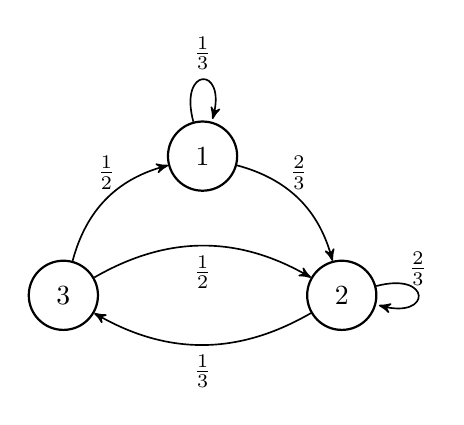
\begin{tikzpicture}[->, >=stealth', auto, semithick, node distance=2.5cm]
\tikzstyle{every state}=[fill=white,draw=black,thick,text=black,scale=1]
\node[state]    (A)               {$1$};
\node[state]    (B)[below right of=A]   {$2$};
\node[state]    (C)[below left of=A]   {$3$};
\path
(A) edge[bend left, above]    node{$\frac23$}   (B)
    edge[loop above, above]    node{$\frac13$}  (A)
(B) edge[bend left, below]    node{$\frac13$}   (C)
    edge[loop right, above]    node{$\frac23$}  (B)
(C) edge[bend left, above]    node{$\frac12$}   (A) 
    edge[bend left, below]    node{$\frac12$}   (B);
\end{tikzpicture}
\end{center}
\caption{Discretizing our continuous markov chain}
\end{figure}

This alllows us to compute a stationary distribution according to the transition matrix 
\[ P = \bbm \frac13 & \frac23 & 0 \\ 
            0       & \frac23 & \frac13 \\ 
            \frac12 & \frac12 & 0 \ebm 
        \] 
        And now if you solve for $\pi P = \pi$, you'll get the same exact answer that we had before. Neat. 

\subsection{Random Graphs}
We're stealing from MIT again, since their 6.207/14.15 notes are pretty good (who would've thought). It's actually a graduate course in economics, so it's interesting to see how probability theory still shows up in far away fields. 

First off, there's lots of applications to the behavior of social networks, biological networks, matrix completion, etc. Some examples are understanding if a population will become extinct or if an epidemic will wipe out all of the species. 

\begin{definition}
The models of random graphs we will use are called \textbf{Erdos-Renyi} Random Graphs. We denote them by $\Gcal(n,p)$ where $n$ is the number of vertices, and $p$ is the probability of an edge being present or not. Typically $n\in \ZZ^+$, $0\leq p \leq 1$.
\end{definition}

Here's one way to view this. Flip a coin for every edge to determine if its present. This is independent for each edge in the graph. 

We can ask some preliminary questions about random graphs, such as... 

\begin{question}
    What is $\EE[\text{\# of edges}]$?
\end{question}
\begin{proof}[Answer]
    Using linearity of expectation, $\EE[\text{\# of edges}] = \binom{n}{2}p = \frac{n(n-1)}{2}p$. 
\end{proof}

\begin{question}
    What is the distribution  of $D$, the degree of a node? What is $\EE[D]$? 
\end{question}
\begin{proof}[Answer]
    There's $n-1$ potential other edges, each of which will have probability $p$ of appearing. The density is $p_D(d) = \binom{n-1}{p} p^d(1-p)^{n-1-d}$. Hence $D\sim \Bin(n-1, p)$, so $\EE[D] = (n-1)p$.  
\end{proof}

\begin{question}
    If $n\to\infty, p\to 0$ while $(n-1)p = \la$ is a constant, how do you approximate $p_D(d)$? 
\end{question}
\begin{proof}[Answer]
    We approximate $D$ as $\Poisson(\la)$, so $p_D(d) \approx e^{-\la}\dfrac{la^d}{d!}$. 
\end{proof}

\begin{question}
    What is the probability $q$ that a node is isolated? 
\end{question}
\begin{proof}[Answer]
    All edges must not be present, so $q = (1-p)^{n-1}$. 
\end{proof}

Erdos and Renyi stated a number of results that are based on ``thresholds'' of $p$ needed for certain \emph{structural properties} of the graph to emerge. 

\begin{example}[Structural Properties]
    Here's some examples of what we mean by structural properties. Note that all of these properties occur in the limit $n\to \infty$.
    \begin{itemize}
        \ii $p = \frac{1}{n^2}$ is a threshold for when the first edge appears w.h.p.
        \ii $p = \frac{1}{n}$ is a threshold for a ``Giant Component'' to emerge. That is, if $p = \frac{1-\epsilon}{n}$, we will have lots of small components (much like raindrops) of size $O(\log n)$. On the other hand, if $p = \frac{1+\epsilon}{n}$, then we will still have a few small components, but there will also be a ``Giant Component'' of size $O(n)$. 
        \ii We will focus on perhaps the most important property: a threshold for \textbf{connectedness}, which is $p = \frac{\log n}{n}$.  
    \end{itemize}
\end{example}

In all of our random graph ventures, we pick an $n$, then pick a $p$ based on what $n$ is. Hence all of our $p$ will implicitly be functions of $n$. We assume you know this, so for convenience sake we drop the notation. Now let's prove this last property. 

\begin{theorem}[Erdos-Renyi 1961]
    Let $p(n) = \la\frac{\log n}{n}$. Then, 
    \alphanum
        \ii If $\la < 1$, $\PP(\Gcal(n,p) \text{ is connected})\to 0$ as $n\to\infty$.
        \ii If $\la > 1$, $\PP(\Gcal(n,p) \text{ is connected})\to 1$ as $n\to\infty$.
    \enumend
    \label{thm:connected}
\end{theorem}
Quick remark: this should remind you of Shannon's capacity theorem. If the capacity is anything less than the maximum, you will eventually transmit all of your message with positive probability. Otherwise, you will never be able to. Same on-off principle.

\begin{proof}
    We will prove part (a) first, opting to prove something stronger. It suffices to show that $\PP(\text{no isolated nodes}) \to 0$ as $n\to\infty$. 

    Let $X$ be the number of isolated nodes in $\Gcal(n,p)$. Let's find $\EE[X]$. We use our old friend indicator variables, letting $I_i$ be an indicator that $i$ is isolated. Then, 
    \[ \EE[X] = \sum_{i = 1}^n \EE[I_i] = \sum_{i = 1}^n \PP(\text{node }i\text{ is isolated}) = nq\] 
    where $q$ is from our preliminary excursion above. Thus, 
    \[ \EE[X] = nq = n(1-p)^{n-1} \approx ne^{-p(n-1)} \approx ne^{-np} = n e^{-\la\log n} = n^{1-\la}.\] 
    The first approximation was just a Taylor Series approximation, while the second one assumes that $e^p \approx 1$, which is true as $p\to 0$. Hence, for any constant $\la$, our expectation blows up as $n\to \infty$, which is really good, since we want $\PP(X = 0) = 0$. 

    But is this enough? Is knowing that our expectation goes to infinity enough to state that there is no mass at $0$? 

    Turns out its not, and one can create bad eamples where this happens. For example, we can have a variable $R$ for which $\PP(R = 0) = \frac{1}{n}$ and $\PP(R = n^2) = \frac{n-1}{n}$. Expectation goes to infinity, but we still have remaining mass at $0$. 

    To fix this, we need to control the variance as well. This is kind of annoying, but there's a nice easy lemma we can make use of. 

    \begin{lemma}
        If $X$ is a nonnegative integer valued RV, then $\PP(X = 0) \leq \dfrac{\Var(X)}{[\EE[X]]^2}.$ 
    \end{lemma}
    \begin{proof}
        We have 
        \begin{align*}
            \Var(X) &= \EE[(X - \EE[X])^2] \\
                    &= \PP(X = 0)\EE[X]^2 + \PP(X=1)\EE[(X-1)^2] + \PP(X=2)\EE[(X-2)^2] + \dots \\ 
                    &\geq \PP(X= 0) \EE[X]^2.
        \end{align*}
        from which the result follows. 
    \end{proof}
    
    Hence if we can show that the variance goes to $0$, then so does $\PP(X = 0)$. Expanding results in 
    \begin{align*}
        \Var(X) &= \Var\left(\sum_{i=1}^n I_i\right) = \sum_{i=1}^n \Var(I_i) + \sum_{i\not= j} \Cov(I_i, I_j)  \\ 
                &= n\Var(I_i) + n(n-1)\boxed{\Cov(I_1, I_2)}.
    \end{align*}
    We can treat $I_i$ as a Bernoulli random variable with probability $q$ of being $1$, from which $\Var(I_i) = q(1-q)$.

    All we have left to calculate is the boxed portion, the covariance, which is 
\[ \Cov(I_1, I_2) = \EE[I_1I_2] - \EE[I_1]\EE[I_2].\] 
The first quantity asks for the probability that two nodes are both isolated. This requires all $2(n-1)-1 = 2n-3$ edges out of both nodes to be absent, giving a probability of $(1-p)^{2n-3}$. 

The second quantity was already calculated earlier. If $q = (1-p)^{n-1}$ is the probability that a node is isolated, the product is just $q\cdot q = q^2$. Putting this all together, 
    \[\Cov(I_1, I_2) = \frac{q^2}{1-p} - q^2 = \dfrac{pq^2}{1-p}.\] 
    So our variance is 
    \[ \Var(X) = nq(1-q) + \dfrac{n(n-1)pq^2}{1-p}.\] 
    Finally, we can use our lemma (along with $\EE[X] = nq$) to show that 
    \[ \PP(X = 0) \leq \dfrac{\Var(X)}{\EE[X]^2} = \dfrac{1-q}{nq} + \dfrac{(n-1)p}{n(1-p)} \to 0\] 
    as $n\to \infty$, completing our proof. 
\end{proof}

\newpage
\section{Thursday, April 4th}
Thanks to Megan Kawakami for her notes on this day. 

\subsection{More on Random Graphs}
Recall from last lecture that we were discussing random graphs, and how they could be used to prove many \emph{structural properties} of graphs. One of these is that of connectedness in graphs which is described by Theorem~\ref{thm:connected}. We will reinterpret the theorem as follows. 

Suppose we have a random graph $\Gcal(n, p)$ where $p(n) = \frac{\la\log n}{n}$. Then our two threshold scenarios can be described as follows: 
\alphanum
    \ii If $\la < 1$, then $\PP(\text{no isolated nodes}) \to 0$ as $n\to\infty$.
    \ii If $\la > 1$, then $\PP(\text{not connected}) \to 0$ as $n\to\infty$. 
\enumend

We proved part (a) last lecture previously, so now we will prove part (b). Before we do so, recall from the proof of part (a) that if $X$ is the number of isolated nodes in $\Gcal(n, p)$, then $\EE[X] = nq \approx n^{1-\la} \to \infty$ as $n\to\infty$. 

\begin{proof}[Proof of part (b)]
    We will prove the converse; if $\la > 1$, then $\PP(\text{connected}) \to 1$. 

    The key idea is that a graph being disconnected is equivalent to the existence of a set of size $k$ (where $1\leq k \leq \frac{n}{2}$) such that there's no edge between this set and its complement. Using this idea, we can find the probability of the latter event and use the union bound to upper bound our probability: 

    \begin{align*}
        \PP(\Gcal(n,p)\text{ is not connected}) 
        &= \PP\left(\bigcup_{k=1}^{\frac{n}{2}} \{\exists\text{ a set of size }k\text{ that is disconnected from its comp set}\}\right) \\ 
        &\leq \sum_{k=1}^{\frac{n}{2}} \PP(\exists\text{ a set of size }k\text{ that's disconnected}) \\ 
        &\leq \sum_{k=1}^{\frac{n}{2}} \dbinom{n}{k} \PP(\text{a specific set of }k\text{ nodes is disconnected from comp}) \\ 
        &= \sum_{k=1}^{\frac{n}{2}} \dbinom{n}{k} (1-p)^{k(n-k)}
    \end{align*}
    where the last step follows since the $k(n-k)$ cross edges between components need to all be missing, which happens individually with probability $1-p$. Through some tedious calculations with non-obvious inequailty bounds, we can show that this last summation goes to 0, as desired. 

    As a specific example, take $k = 1$. Then we have 
    \[ \dbinom{n}{1} (1-p)^{n-1} = \EE[X] \approx ne^{-p(n-1)} \approx n^{1-\la} \xrightarrow{n\to\infty} 0.\] 
\end{proof}

\subsection{Inference: Detection and Bayes' Rule}

There are two main approaches to performing inference. One is the \emph{classical} or \emph{frequentist} approach, where the unknowns are fixed and to be estimated. The other is the \emph{Bayesian} approach, where the unknowns are RVs whose distributions have to be estimated. Each of these will lead to a different inference method as we will see later. 

The basic premise is that we have $n$ possible exclusive causes $C_1, C_2, \dots, C_n$ of a particular symptom. Each cause has a prior probability $p_i$ and it has a probability $q_i$ of causing the symptom. We call $p_i$ our \emph{priors} and $q_i$ our \emph{posteriors}, and can illustrate the setup with the following diagram. 

\begin{figure}[!htb]
    \centering
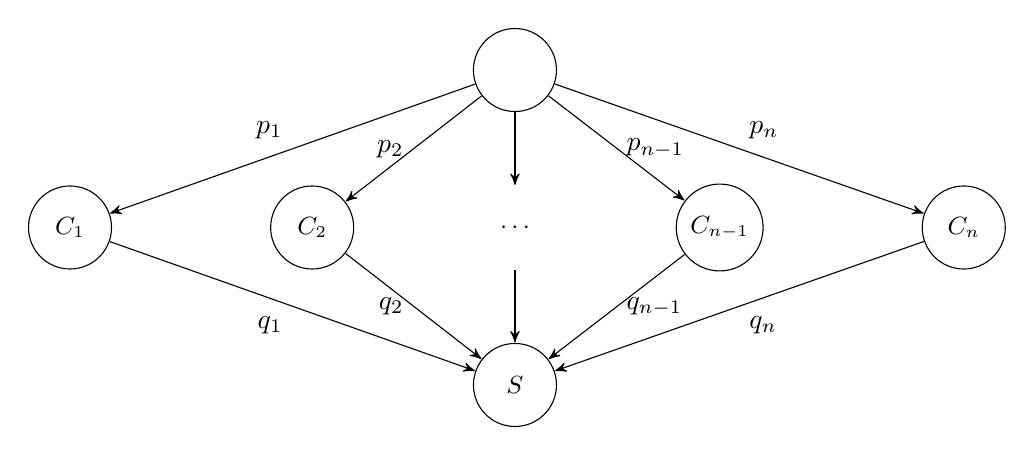
\begin{tikzpicture}
  \tikzset{
    ->, 
    >=stealth',
    semithick, 
    node distance=2cm,
    state/.style={minimum size=30pt,font=\small,circle,draw},
    dots/.style={state,draw=none},
    %edge/.style={->},
  }
  \node [state] (0)                    {};
  \node [dots] (cm)  [below of = 0]   {$\cdots$}; 
  \node [state] (c2)  [left=1.5cm of cm]   {$C_2$};
  \node [state] (c1)  [left=2cm of c2]  {$C_1$};
  \node [state]  (cd)  [right=1.5cm of cm]  {$C_{n-1}$}; 
  \node [state] (cn)  [right=2cm of cd]  {$C_n$}; 
  \node [state] (1)   [below of = cm]  {$S$}; 

  \path
  (0) edge[above left]    node{$p_1$}   (c1)
      edge[left]    node{$p_2$}   (c2)
      edge[below]    node{}        (cm)
      edge[right]   node{$p_{n-1}$}   (cd)
      edge[above right]    node{$p_n$}   (cn)
  (c1) edge[below left]   node{$q_1$}   (1)
  (c2) edge[left]   node{$q_2$}   (1)
  (cm) edge[below]   node{}        (1)
  (cd) edge[right]   node{$q_{n-1}$}        (1)
  (cn) edge[below right]   node{$q_n$}   (1); 
\end{tikzpicture}
\caption{The basic inference setup, where the $C_i$'s are possible causes of a symptom $S$.}
\label{fig:map}
\end{figure}

Suppose we want the posterior probability $\pi_i$ of cause $i$ given the symptom $S$. In other words, the probability that cause $i$ caused the symptoms we observed. Then we can use Bayes' Rule to get 
\[ \pi_i  = \PP(C_i | S) = \dfrac{\PP(S | C_i) \PP(C_i)}{\sum_{j=1}^n \PP(S|C_j)\PP(C_j)} = \dfrac{p_iq_i}{\sum_{j=1}^n p_jq_j}. \]

This is important enough to be stated as a theorem. 

\begin{theorem}[Posterior Probability]
    The posterior probability $\pi_i$ of a cause $i$ is given by 
    \[ \pi_i = \dfrac{p_iq_i}{\sum_j p_j q_j}.\] 
\end{theorem}

\subsection{Inference: MAP and MLE, and the MAP Rule}
There are two main inference methods: MAP and MLE. 

\begin{definition}[MAP]
    The \textbf{maximum a posteriori}, or MAP, is defined to be 
    \[ \MAP = \arg\max_i \pi_i = \arg\max_i p_iq_i.\]  
    In other words, it is the best estimate of the cause given a symptom. 
\end{definition}

\begin{definition}[MLE]
    The \textbf{maximum likelihood estimate}, or MLE, is defined to be 
    \[ \MAP = \arg\max_i q_i,\] 
    which is just the MAP estimate under a uniform prior, i.e. $p_1 = \dots = p_n$. 
\end{definition}

More generally, 
\[ \MAP[X | Y = y] = \arg\max_x \PP(X = x | Y = y),\] 
which can be interpreted as finding ``which cause best explains the observed symptom,'' and 
\[ \MLE[X | Y = y] = \arg\max_x \PP(Y = y | X = x),\] 
which can be interpreted as finding ``which cause best \emph{generates} the observed symptom.''

Let's do an inference example in digital communications. Suppose we're trying to send a message $X$ across a channel. Unfortunately, the channel is noisy, so the message received is actually $Y$. Given this, our goal is to find an estimate for $X$, $\hat{X}$, given our observation $Y$. In other words, we want to find the MLE and MAP estimate of $X$ given $Y$. 





\newpage
\section{Thursday, April 11th}
Lab 6 is due tomorrow, projects due 4/19, and HW 10 due next Wed. Readings for MLE/MAP are W 5.1-5.4, B\&T 8.1-8.2, 9.1. For Hypothesis Testing, readings are W 5.5,5.6,6.5 and B\&T 9.3-9.4. 

\subsection{Wrap up MLE/MAP}

Recall that the basic premise is that we have $n$ causes and an observed symptoms, and we are trying to perform inference on the causes. Refer to Figure~\ref{fig:map} for more details. Then with this convention, MAP = $\arg\max_{i} p_iq_i$ and MLE = $\arg\max_i q_i$. where $p_i$ are our priors and $q_i$ are the posteriors. Let's see how we could model this in digital communications. 

Suppose we have a Binary Symmetric Channel (BSC). Then using the MAP rule, we can derive a formulation for the likelihood... 

\subsection{Gaussian Channel}
Now suppose we have a setup with a Gaussian channel. Then, 

\[ f_0(y) = \dfrac{1}{\sqrt{2\pi} \sigma}e^{-y^2/2\si^2}.\] 
\[ f_1(y) = \dfrac{1}{\sqrt{2\pi} \sigma}e^{-(y-1)^2/2\si^2}.\] 

Then by MAP, we find 
\begin{align*}
    p_0q_0 &\underset{{1}}{\overset{0}{\gtrless}} p_1q_1 \\ 
    p_0f_0(y) &\underset{{1}}{\overset{0}{\gtrless}} p_1f_1(y).
\end{align*}
We can interpret this as 
%\[\boxed{\dfrac{f_0(y_}{f_1(y)} \underset{{1}}{\overset{0}{\gtrless}} \dfrac{p_1}{p_0}.} \]

We would call the thing on the left the \emph{likelihood} $L(y)$. One thing we can do is take logs to make this easier to evaluate (hence the term \emph{log-likelihood}). This gives 
% WGN channel?

\begin{align*}
    \ln f_0(y) - \ln f_1(y) &\underset{{1}}{\overset{0}{\gtrless}} \ln(\frac{p_1}{p_0}) \\ 
    -\frac{y^2}{2\si^2} + \frac{(y-1)^2}{2\si^2} \grle{0}{1} \ln(\frac{p_1}{p_0}).
\end{align*}

Solving for $y$ gives us a MAP of 
\[ \text{MAP: } \boxed{y \legr{0}{1} \frac{1}{2} + \si^2\ln(\frac{p_0}{p_1})}.\] 
Of course, we can also solve for the MLE, since we just set all of our priors equal, i.e. $p_0 = p_1$. 

\[ \text{MLE: } \boxed{y \legr{0}{1} \frac{1}{2}}.\] 

\begin{example}
    Suppose $\frac{p_0}{p_1} = e$, and $\si^2 = 0.1$. Then our MAP decision would be $y\legr{0}{1} 0.6$.
\end{example}

Read Chapter 5 of Walrand for details of applications to digital communications. 

\subsection{German Tank Problem}
Suppose we have $n$ balls in a bucket, and we're trying to figure out what $n$ is by sampling. Each ball has a serial number from $1$ to $n$. 

Suppose we sample once and get a ball labeled $17$. Then what is the MLE of the maximum serial number in the bucket, $n$? 

It would just be 17, because the probability of getting $17$ if $n < 17$ is 0, and the probability of getting 17 if $n \geq 17$ is $\frac{1}{n}$ which is strictly decreasing.

In other words, $MLE[n | Y_1 = 17] = 17$, since $ML = \arg\max_{i} q_i$. In fact, for any $m = 1, 2, \dots, n$, $\PP(Y = m | X = n) = \frac{1}{n}$, so $MLE[n | Y = m] = m$. 

This is completely against what our intuition says. We should be able to know something more about the total number of balls that's not obvious. 

The problem is that there is a sampling bias that we aren't accounting for in the problem. Suppose we make $k$ observations. There are $\binom{n}{k}$ sets of $k$ distinct $\#$'s that are subsets of $[n] = \{1, 2, \dots, n\}$. Each set is equally likely, so  
\[ \PP_Y(y, n) = \begin{cases} 
\frac{1}{\binom{n}{k}} &\quad\text{ if } n \geq m_k = \max(Y_1, \dots, Y_k) \\         0 & \text{ else}. \end{cases} \] 
    Then the estimator we are using, the maximum likelihood estimation $m_k = \max\{Y_1, Y_2, \dots, Y_k\}$, is actually biased! One can show that $\EE[m_k] \not = n$; in fact, $\EE[m_k] = \frac{k(n+1)}{k+1}$. This is contrary to what we want, since an unbiased estimator should have an expectation equal to the true value. 

    The bias of MLE is $b(M_k) = \EE[M_k] - n = \frac{k-n}{k+1}$. 

    If we want an unbiased estimator, then we could instead use $\hat{N_k} = \frac{k+1}{k} m_k - 1$. Note now that $\EE[\hat{N_k}] = n$ as desired, so this is indeed an unbiased estimator. 

\begin{example}
    Suppose $n = 155$, and we draw $k = 4$ samples. Our samples are $Y = \{ 17, 62, 102, 120\}$. Then $m_k = 120$, so $\hat{N}_k = \frac{5}{4}\cdot 120j - 1 = 149$. 
\end{example}

\subsection{Hypothesis Testing: Neyman-Pearson Test}
The motivation for hypothesis testing is that there are many things that you can't put priors on, like having cancer, or how likely my house is to be on fire. So thinking about them in terms of MLE and MAP isn't the right approach. Alternatively, we have the mindset of giving likelihoods of these events based on our risk-aversion, a.k.a. how tolerant we are to false alarms. 

In general, the setup is as follows: 
\begin{itemize}
    \ii Observe a random variable $Y$. 
    \ii Under hypothesis $H_0$ (i.e. given $X=0$), $Y\sim f( y | 0)$ (no cancer). 
    \ii Under hypothesis $H_1$ (i.e. given $X=1$), $Y\sim f( y | 1)$ (cancer). 
\end{itemize}
Then our goal is to come up with a decision rule $r: \RR\to \{0,1\}$. 

Perhaps the most important formulation is the Neyman-Pearson (N-P) formulation. In it, we have no priors, only two hypotheses, and false negatives are way more important than false positives. 

\begin{figure}[!htb]
\centering

%% include hypotehsis testing graphic
\caption{Table of outcomes based on our decision and the true hypothesis.}
\end{figure}

Our goal is to the maximize PCD, the probability of correct detection, which is $\PP(\hat{x} | X = 1)$ such that the probability of a false alarm, PFA, is $\leq \beta = \PP(\hat{x} | X = 0)$ ($\hat{x}$ is Walrand's way of denoting $r(Y)$). 

The Neyman-Pearson theorem gives us the optimal decision rule for maximizing PCD such that $PFA \leq \beta$. 

\begin{theorem}[Neyman-Pearson]
    The decision $\hat{X}$ that maximized PCD under the constraint that $\text{PFA}\leq \beta$ is 
    \[ 
        \hat{X} = 
        \begin{cases} 
            1 \quad \text{ if } L(Y) > \la \\ 
            0 \quad \text{ if } L(Y) < \la \\ 
            1 \quad \text{ w.p. } \gamma \text{ if } L(Y) = \la 
        \end{cases}
    \]
    where $L(y) = \frac{f_{Y|X}(y|1)}{f_{Y|X}(y|0)}$ is called the \emph{Likelihood Ratio} and $\la > 0$ and $\gamma \in [0,1]$ are chosen to ensure that PFA = $\beta$. 
\end{theorem}

This rule is sometimes called the \emph{threshold rule}. The Neyman-Pearson theorem claims that this rule is \textbf{the most powerful} rule at some PFA $\beta$

\newpage
\section{Tuesday, April 16th}

\subsection{Hypothesis Testing}



\subsection{Estimation: LLSE}


\newpage
\section{Thursday, April 18th}

\subsection{Hilbert Space of Random Variables}

\subsection{Gram Schmidt Process}

\newpage
\section{Tuesday, April 23rd}
HW 11 is due tomorrow, Projects are due on Friday. Reading is chapters 6-8 of Walrand and 8.3-8.5 of B\&T. 

\subsection{LLSE: Recap}
Recall that a Linear Least Squares Estimator (LLSE) is trying to predict a random variable $X$ given some observations $Y$, denoted as $L[X|Y]$. Since the estimator is linear, our predictions are always of the form $\hat{X} = a + bY$; the error of our prediction is $\Delta = X - \hat{X}$. 

We also have that 
\[ L[X|Y] = \EE[X] + \dfrac{\Cov(X,Y)}{\Var(Y)}[Y - \EE[Y].\]

Our LLSE has two properties: 
\begin{enumerate}
    \ii Our estimator is unbiased, i.e. $\EE[\hat{X}] = \EE[X]$. 
    \ii Our error $\Delta$ is uncorrelated with the observation, i.e. $\Cov(\Delta, Y) = 0$.
\end{enumerate}

Makes sense, right? 

Last lecture we also went over interpretations of LLSE in terms of Hilbert space geometry (for zero-mean RVs); this allows us to do geometric things with random variables. Too bad it was erased before I could get it down rip. There's notes on the website however.  

Using this interpretation, the LLSE is just the projection of $X$ onto $Y$, so 
\[ L[X|Y] = \proj_{Y}X = \dfrac{\cyc{X,Y}}{||Y||^2} Y = \dfrac{\EE[XY]}{\Var(Y)}Y.\] 

\begin{example}
    Let $Y = X + Z$, where $X$ and $Z$ are independent and zero-mean. What is $L[X|Y]$? 
\end{example}
\begin{proof}[Solution]
    Knowing that they're zero-mean allows us to use the geometric interpretation of LLSE, which is just the projection. 

    Let this projection be $bY$ (since it lies on the vector $Y$). Then by similar triangles (we have right angles since $X,Y$ have covariance 0), 
    \[ \dfrac{||b\vec{Y}||}{||X||} = \dfrac{||X||}{||Y||} \implies ||bY|| = \dfrac{||X||^2}{||Y||} = \]
\end{proof}

We can also ask what the error would be. By using similar triangles again, 
    \[ \dfrac{||\Delta||^2}{||X||^2} = \dfrac{||Z||^2}{||Y||^2}.\] 

\subsection{Linear Regression}
Let's take a look at Linear Regression from a Non-Bayesian view. So far, we have assumed a Bayesian framework (i.e. joint distribution of $X,Y$ are known), but instead let's take a ``data-driven'' perspective.  

Suppose we have access to $(X_1, Y_1), (X_2, Y_2), \dots, (X_k, Y_k)$. Our goal is to construct $g(Y) = a + bY$ so that 
\[ \dfrac{1}{k} \sum_{i = 1}^k |X_i - (a + bY_i)|^2\]
is minimized. This makes sense since our observations are $Y$, so given them we want to predict the original values, namely $X$. 

It's also important to note that this is just a special case of the Bayesian approach, where each of our $k$ data points is equally likely, and hence has a prior of probability $\frac{1}{k}$. Hence $(X,Y) \sim \Uniform\{(x_i, y_i)_{i=1}^k\}$. So minimizing our error is equivalent to solving 

\[ \xi(a,b) = \dfrac{1}{k}  \sum_{i = 1}^k |X_i - (a + bY_i)|^2 \implies \dfrac{\pd\xi}{\pd a} = 0, \dfrac{\pd\xi}{\pd b} = 0.\] 

Our estimator then is just 
\[ a + bY = \EE_k[X] + \dfrac{\Cov_k(X,Y)}{\Var_k(Y)} (Y - \EE_k(Y)).\] 

But $\EE_k[X] = \frac{1}{k} \sum_{i=1}^k X_i$ and $\EE_k[Y] = \frac{1}{k}\sum_{i=1}^k Y_i$. Also 
\[ \Var_k(Y) = \frac{1}{k} \sum_{i=1}^k Y_i^2 - \EE_k^2[Y] \] 
and 
\[ \Cov_k(X,Y) = \frac{1}{k} \sum_{i=1}^k X_iY_i - \EE_k[X] \cdot \EE_k[Y].\] 

By SLLN, as $k\to \infty$, Linear Regression approaches the LLSE estimator. 

This Linear Regression is also the same as the one we did in 16A and all your fancy ML classes. The linear algebra perspective is that we want to solve for $x$ in $Ax = b$, where in this case, 

\[ \bbm 
    1 & Y_1 \\ 
    1 & Y_2 \\ 
    \vdots & \vdots \\ 
    1 & Y_k 
    \ebm
    \colvec{2}{a}{b} 
    = 
    \colvec{4}{X_1}{X_2}{\vdots}{X_k}
\] 
Least squares says that the solution is $x = (A^TA)^{-1}A^T b$. You can actually convince yourself that $\hat{X}_{LS} = \colvec{2}{a}{b}$, where $a,b$ are the same covariance/expectation values as from the Bayesian framework. So the approaches are equivalent, except our LLSE Bayesian approach gives us more generality. 

\subsection{MMSE}
We can move up to higher degree estimators, such as $\hat{X} = a + bY + cY^2$, and you can imagine that doing so will give you better results. But you run the risk of overfitting to your data. 

%Let's take a step back and think about this from a Bayesian perspective. 

Instead of constraining ourselves as before to linear estimate models, we now simply want the best mean squared estimator. Assume you know the joint pdf of $X,Y$. Our goal is to find $g(Y)$ such that $\EE[(X - g(Y))^2]$ is minimum. This is what we call the \textbf{Minimum Mean Square Error} estimate, or MMSE estimate. Note that this is over ALL functions $g(Y)$, so this is a pretty hard problem. 

Suppose we knew nothing about the data. Then the best value we could pick is just the mean of the data (you can convince yourself why this minimizes the mean squared error). Now suppose we conditioned on $Y = y$; by the same logic, we should just pick the mean of the data where $Y = y$, which is precisely $\EE[X | Y = y]$. It turns out that this is actually the optimal MMSE, which we will prove.  

\begin{figure}[!htb]
    \centering
    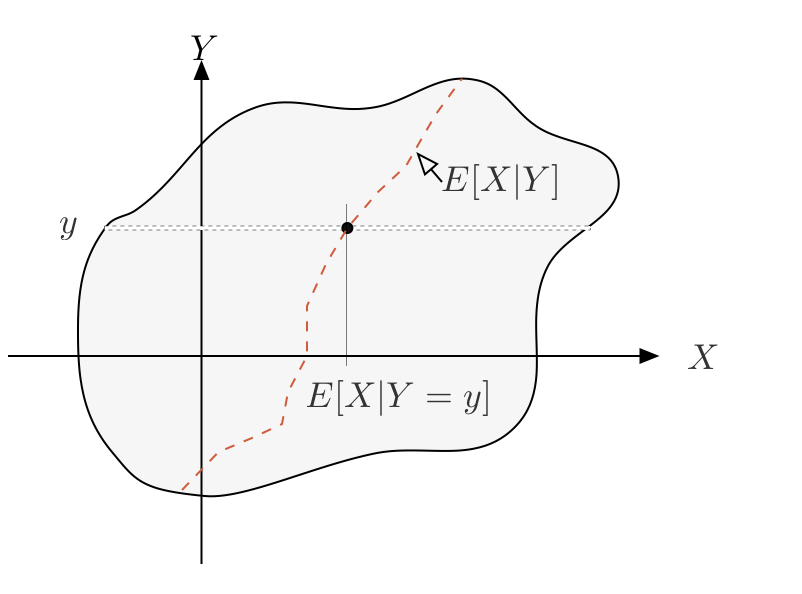
\includegraphics[scale=0.6]{MMSE.png}
    \caption{For a given $y$, $\EE[X|Y=y]$ is just the mean of the mass where $Y=y$. Source: Walrand.}
\end{figure}

\begin{theorem}[Walrand 7.4]
    The minimum mean squares error estimate is 
    \[ \MMSE[X|Y] = \EE[X|Y],\] 
    where 
    \[ \EE[X|Y = y] = \int_{-\infty}^\infty x f_{X|Y}(x|y) dx.\] 
\end{theorem}

Before we start, we will need some lemmas that we state without proof. 

\begin{lemma}[Walrand 7.6]
    For any function $\phi(\cdot)$, 
    \alphanum
        \ii $\EE[(X - \EE[X|Y])\cdot \phi(Y)] = 0$; in other words, $\Delta = X - \EE[X|Y]$ is independent of $\phi(Y)$ for all $\phi(\cdot)$.  
        \ii If $\exists g(Y)$ such that $\EE[(X - g(Y))\cdot \phi(Y)] = 0$ for all $\phi(\cdot)$, then $g(Y) = \EE[X | Y]$. 
    \enumend
\end{lemma}

\begin{proof}[Proof of Theorem 7.4]
    Let $G(Y) = \{ g(Y) | g(\cdot) \text{ is a function}\}$ be the space of all functions on $Y$. 

    As with the LLSE, $X - \EE[X|Y]$ is independent to the projection of $X$ on to a general member of the functional space, say $h(Y)$. Now if we could show that 
    \[ \EE[|X - h(Y)|^2] \geq \EE[|X - \EE[X|Y]|^2|],\] 
    then we're done, since this shows that no matter what functional you pick, $\EE[X|Y]$ is always king. 

    So let's take the left hand side and expand it using the world's most \emph{annoying} trick, adding and subtracting some quantity. 
    \begin{align*}
        \EE[|X - h(Y)|^2] &= \EE[|X - \EE[X|Y] + \EE[X|Y] - h(Y)|^2] \\ 
                          &= \EE[|X - \EE[X|Y]|^2] + \EE[|\EE[X|Y] - h(Y)|^2] + 2\EE\left[(X - \EE[X|Y])(\EE[X|Y] - h(Y))\right]
    \end{align*}
    Here's the slick part though; since $\EE[X|Y]$ and $h(Y)$ both belong to $G(Y)$, their difference is still a function of $Y$, so $\phi(Y) = \EE[X|Y] - h(Y) \in G(Y)$. So by part (a) of our lemma, the product is just 0.

    Also, our second term is always nonnegative since it's the expected value of something squared, so 
    \[ \EE[|X - h(Y)|^2] = \EE[|X - \EE[X|Y]|^2] + \EE[|\EE[X|Y] - h(Y)|^2] \geq \EE[|X - \EE[X|Y]|^2] \] 
    and so we're done. 
\end{proof}

\subsection{Jointly Gaussian}
In general, our MMSE won't be the same as our LLSE, since the projection of $X$ onto the general space $G(Y)$ won't be the same as our projection onto $a + bY$, which is a subspace of that general space. In other words, $L[X|Y] \not= \EE[X|Y]$. 

So when are they equal then? One case is obvious; when $g(Y)$ is linear. But if you think about it more generally, this will always hold when $X$ and $Y$ are \emph{jointly Gaussian}, or JG. 

This is really important, since the main problem with the MMSE is that finding it numerically is extremeley tough. But if $X,Y$ are jointly Gaussian, we can use our formula for the LLSE from before. This is big enough to be stated as a theorem. 

\begin{theorem}[Walrand 7.8]
    If $(X,Y)$ are jointly Gaussian, then 
    \[ \EE[X|Y] = L[X|Y]  = \EE[X] + \dfrac{\Cov(X,Y)}{\Var(Y)} (Y - \EE[Y]).\] 
\end{theorem}

What does being Jointly Gaussian mean? It means that $X = (X_1, X_2)$ has a multivariate normal pdf. 

\newpage
\section{Thursday, April 25th}

\subsection{Jointly Gaussian Random Variables}

\subsection{Kalman Filtering}

\newpage 
\section{Tuesday, April 30th}

\subsection{Kalman Filter}


\newpage
\section{Thursday, May 2nd}
Last lecture ~woo~

HW 12 and Lab 7 are due tomorrow, and an optional lab is due next Friday. Stay tuned for review sections. 

\subsection{Hidden Markov Models}
Suppose we had a Markov Model or Chain, but some of the states are hidden to us. In other words, there are states we can't observe, and those we can. Then we call this a \textbf{Hidden Markov Model} since some states are ``hidden''\footnote{Sometimes we refer to them as \textit{latent} as well.} from us, and depict it as such. The $X_i$ are state variables and belong to a state space $\mathcal{X}$ (discrete or continuous), while the $y_i \in \mathcal{Y}$, which also may or may not be discrete. 

\begin{figure}[!htb]
    \centering
    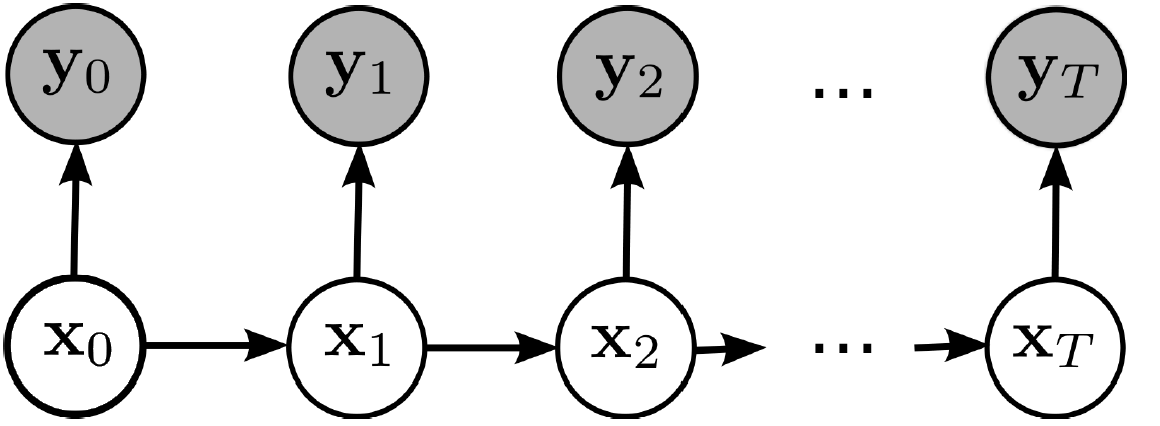
\includegraphics[scale = 0.2]{hmm.png} 
    \caption{A Hidden Markov Model. The grey states are observed, while the white ones are hidden.}
\end{figure}

\begin{example}
    If we had $T = 2$, then the joint probability $\PP(x_0, y_0, x_1, y_1)$ would be 
    \[ \PP(x_0, y_0, x_1, y_1) = \PP(x_0) \PP(y_0 | x_0) \PP(x_1 | x_0, y_0) \PP(y_1 | x_1, x_0, y_0) = \PP(x_0) \PP(y_0 | x_0) \PP(x_1 | x_0) \PP(y_1 | x_1).\]

    Notice that due to the structure of the HMM, we can simplify our probabilities a lot. This will be very useful! (This is akin to how the power of a Markov Chain is that the joint distribution is modeled by just a transition matrix $P$). 
\end{example}

In general, 
\[ \PP(x_0, x_1, \dots, x_n, y_0, y_1, \dots, y_n) = \pi_0(x_0) Q(x_0, y_0) P(x_0, x_1) Q(x_1, y_1) \dots P(x_{n-1}, x_n) Q(x_n, y_n)\] 

where $\pi_0$ is our initial state, $Q$ models our transition probabilities between hidden states and observations, and $P$ models transitions between hidden states. 

Our goal is to find the MLSE, or maximum likelihood sequence estimate, based on our observations $y_0, \dots, y_n$. In other words, we want 

\[ MAP[X^n | Y^n = y^n] \implies \begin{cases} \text{infer the best sequence of (hidden) states} \\ \text{that best explain the observed sequence.} \end{cases} \]

What's one application of Hidden Markov Models and finding the MLSE? Speech Recognition. You receive sounds as observations, and your goal is to find the most likely sequence of words corresponding to the sounds. 

HMMs are super flexible, so there's a couple of ways we can use them depending on what you are trying to find. 

\begin{itemize}
    \ii \textbf{Filtering}: We feed in $Y_0, Y_1, \dots, Y_T$ to our filter and expect out $\hat{X}_T$, the last hidden state. Think Kalman filtering. 

    \[ Y_0, Y_1, \dots, Y_T \rightarrow \boxed{\text{Filter}} \rightarrow \hat{X}_T\] 

    Some examples are tracking positions in real time or monitoring current health of patient given symptoms $\{Y_0\}_{i=0}^T$. 

    \ii \textbf{Prediction}: We feed in $Y_0, Y_1, \dots, Y_T$ and want to predict $\hat{Y}_{T+1}$. 
    
    \[ Y_0, Y_1, \dots, Y_T \rightarrow \boxed{\text{Predict}} \rightarrow \hat{Y}_{T+1}\] 

    Some examples are radar tracking, stock price predictions, or predictive coding (?). 

    \ii \textbf{Smoothing}: We feed in $Y_0, Y_1, \dots, Y_T$ and want to find $\hat{X}_t$ for a choice of $t \leq T$. In other words, if I gave you a value $t$, what is the most likely value of $\hat{X}_t$ given our observations? 

    \[ Y_0, Y_1, \dots, Y_T \rightarrow \boxed{\text{Smooth}} \rightarrow \hat{X}_t \quad t\leq T\] 
    
    Some examples are inferring the cause of a car-crash or ``post-mortem'' analysis. 

    \ii \textbf{MLSE}: We feed in $Y_0, Y_1, \dots, Y_T$ and want the most likely \emph{sequence} $\hat{X}_0, \hat{X}_1, \dots, \hat{X}_T$ that explains our observations. This differs from smoothing, where we only care about maximizing over a single hidden state. 

    \[ Y_0, Y_1, \dots, Y_T \rightarrow \boxed{\text{MLSE}} \rightarrow \{\hat{X}_0, \hat{X}_1, \dots, \hat{X}_T\} \]

    Some examples are speech recognition, auto-correction, and convolutional coding (Viterbi algorithm).
\end{itemize}

We're focusing on just the last one today (MLSE), both to preserve one's sanity but also because time isn't a construct and very realistically limits us. 

\subsection{The Viterbi Algorithm}

Let's now try to write out what the MLSE would be algebraically. We're looking for 

\begin{align*}
    x^{n^*} &= \arg\max_{x^n \in \mathcal{X}^n} \PP[X^n = x^n | Y^n = y^n] \\ 
            &= \arg\max_{x^n} \left[ \pi_0  Q(x_0, y_0) P(x_0, x_1) Q(x_1, y_1) \dots P(x_{n-1}, x_n) Q(x_n, y_n) \right].
\end{align*}

But I don't like taking arg maxes of products, so I'll make an easy fix by taking logs on both sides. 

\[ x^{n^*} = \arg_{x^n\in\mathcal{X}^n}\max \left[ \log \pi_0(x_0) Q(x_0, y_0) + \sum_{m=1}^n \log\left[P(x_{m-1}, x_m) Q(x_m, y_m) \right]\right] .\]

So we've reduced the MLSE problem to optimizing over the right hand side. To make it more compact, let's define 
\begin{align*}
    d_0(x_0) &= -\log \pi_0(x_0)Q(x_0, y_0) \\ 
    d_m(x_{m-1}, x_m) &= -\log\left[ P(x_{m-1}, x_m) Q(x_m, y_m)\right]
\end{align*}

so that all the $d_i's$ are positive (why?). 

Then we have the following. 

\begin{definition}[MLSE]
    Our maximum likelihood sequence estimate reduces to the optimization problem:
    \[ x^{n^*} = \arg\min_{x^n} \left[ d_0(x_0) + \sum_{m=1}^n d_m(x_{m-1}, x_m)\right]  \]
    where $x^{n^*}$ is the optimal sequence explaining our observations. 
\end{definition}

Since things are getting very abstract, we're going to turn to an example to ground our intuition. Ah, good 'ol engineering maths. 

Say you're at a ``nearly honest casino'' which uses a fair die most of the time, but switches to a loaded die occasionally. We can model their transitions ($P$) between using the fair die and the loaded die as the following Markov Chain (so assume we know these parameters).

\begin{figure}[!h]
\begin{center}
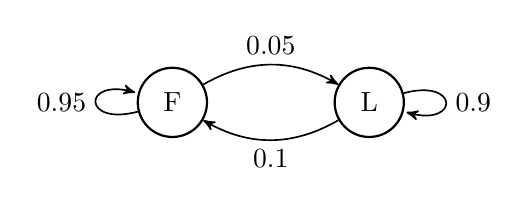
\begin{tikzpicture}[->, >=stealth', auto, semithick, node distance=2.5cm]
\tikzstyle{every state}=[fill=white,draw=black,thick,text=black,scale=1]
\node[state]    (A)               {F};
\node[state]    (B)[right of=A]   {L};
\path
(A) edge[bend left, above]    node{$0.05$}   (B)
    edge[loop left, left]    node{$0.95$}  (A)
(B) edge[bend left, below]    node{$0.1$}   (A)
    edge[loop right, right]    node{$0.9$}  (B);
\end{tikzpicture}
\end{center}
\caption{Transitions for the casino.}
\end{figure}

Additionally, we know that for the fair die, the probability of each outcome is equally likely (as expected), so $\PP(F = i) = \frac{1}{6}$ for $i = 1, \dots, 6$. For the loaded die, we know that $\PP(L = 6) = \frac{1}{2}$ and $\PP(L = 1) = \dots = \PP(L = 5) = \frac{1}{10}$ so that the die is biased towards rolling a 6. 


Then given an observed sequence of die rolls (say $6, 6, 1, 6, 2, \dots$), we want to infer the most likely sequence of ``hidden'' states (say $F, F, L, F, L, \dots$). 

We can use a technique called a ``TRELLIS'' diagram, which looks like this: 

\begin{figure}[!htb]
    \centering 
    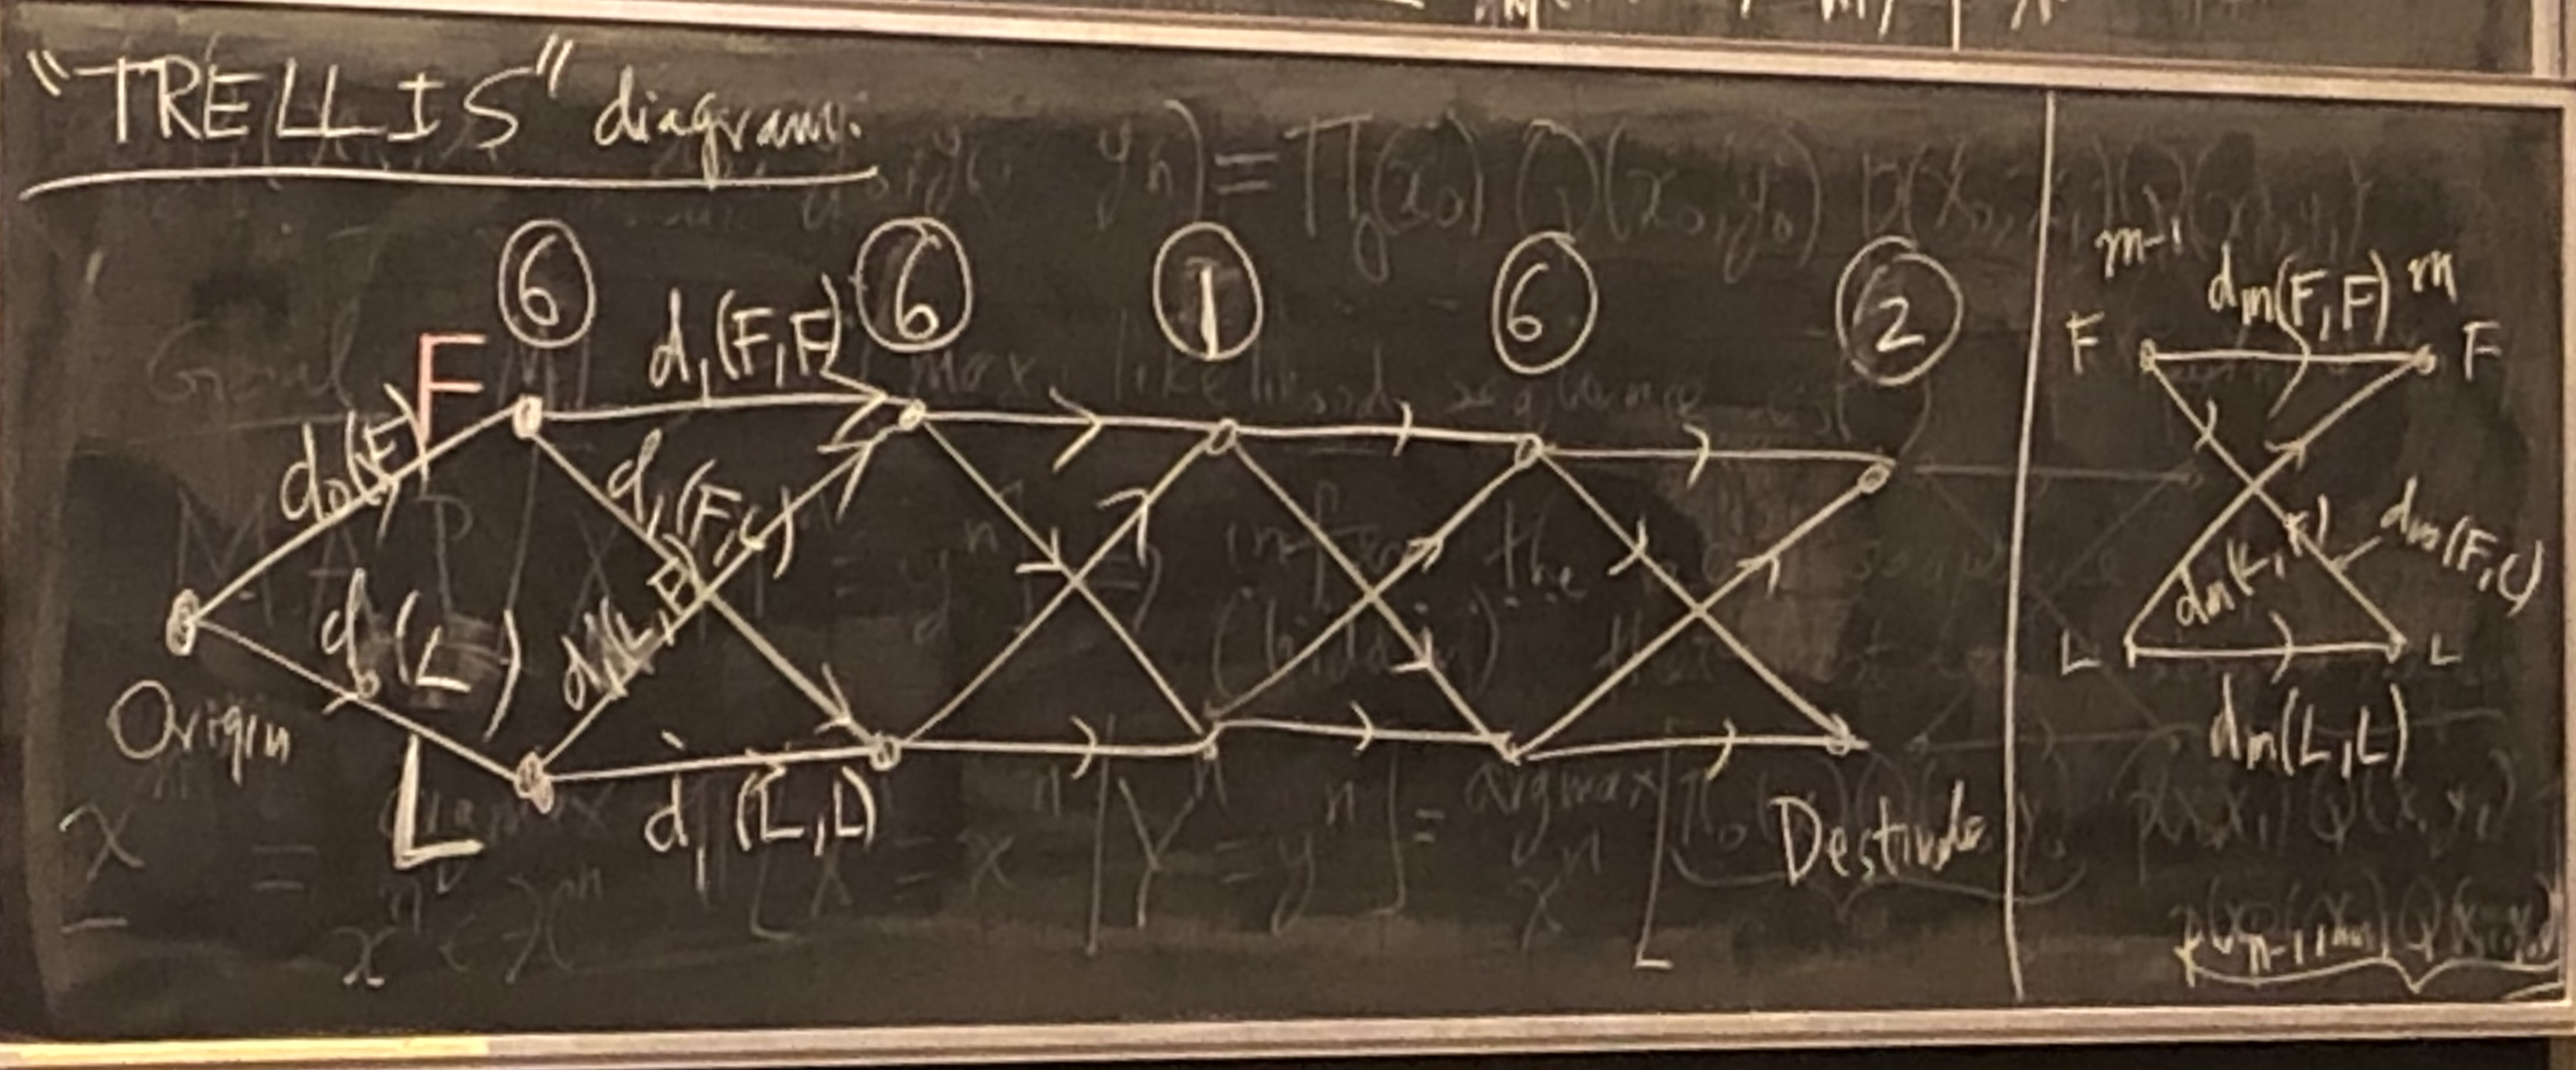
\includegraphics[scale=0.13]{trellis.jpg}
    \caption{A TRELLIS diagram. Looking quite DAG-like.}
\end{figure}

To find the minimum length path from stage $0$ to stage $n$, we just need a good shortest path problem. Bellman-Ford seems like a good choice, especially since its dynamic programming nature lends itself very well to such a calculation (recall that shortest paths on DAGs are best solved by DP). This technique of filling out the diagram using a dynamic programming method is something that Viterbi discovered first, so we call this the \textbf{Viterbi Algorithm}.

First thing's first. We have to calculate our edge weights, a.k.a. all the $d_m$'s. The computation would look something like this: 

\begin{align*}
    d_m(F, F) &= -\log \left[ P(F,F) Q(F, Y_{m})\right] \\ 
    d_m(F, L) &= -\log \left[ P(F,L) Q(L, Y_{m})\right] \\ 
    d_m(L, F) &= -\log \left[ P(L,F) Q(F, Y_{m})\right] \\ 
    d_m(L, L) &= -\log \left[ P(L,L) Q(L, Y_{m})\right] 
\end{align*}

If you plug in those numbers for every possible $m$ based on our observations, your TRELLIS diagram will look something like this: 

\begin{figure}[!htb]
    \centering 
    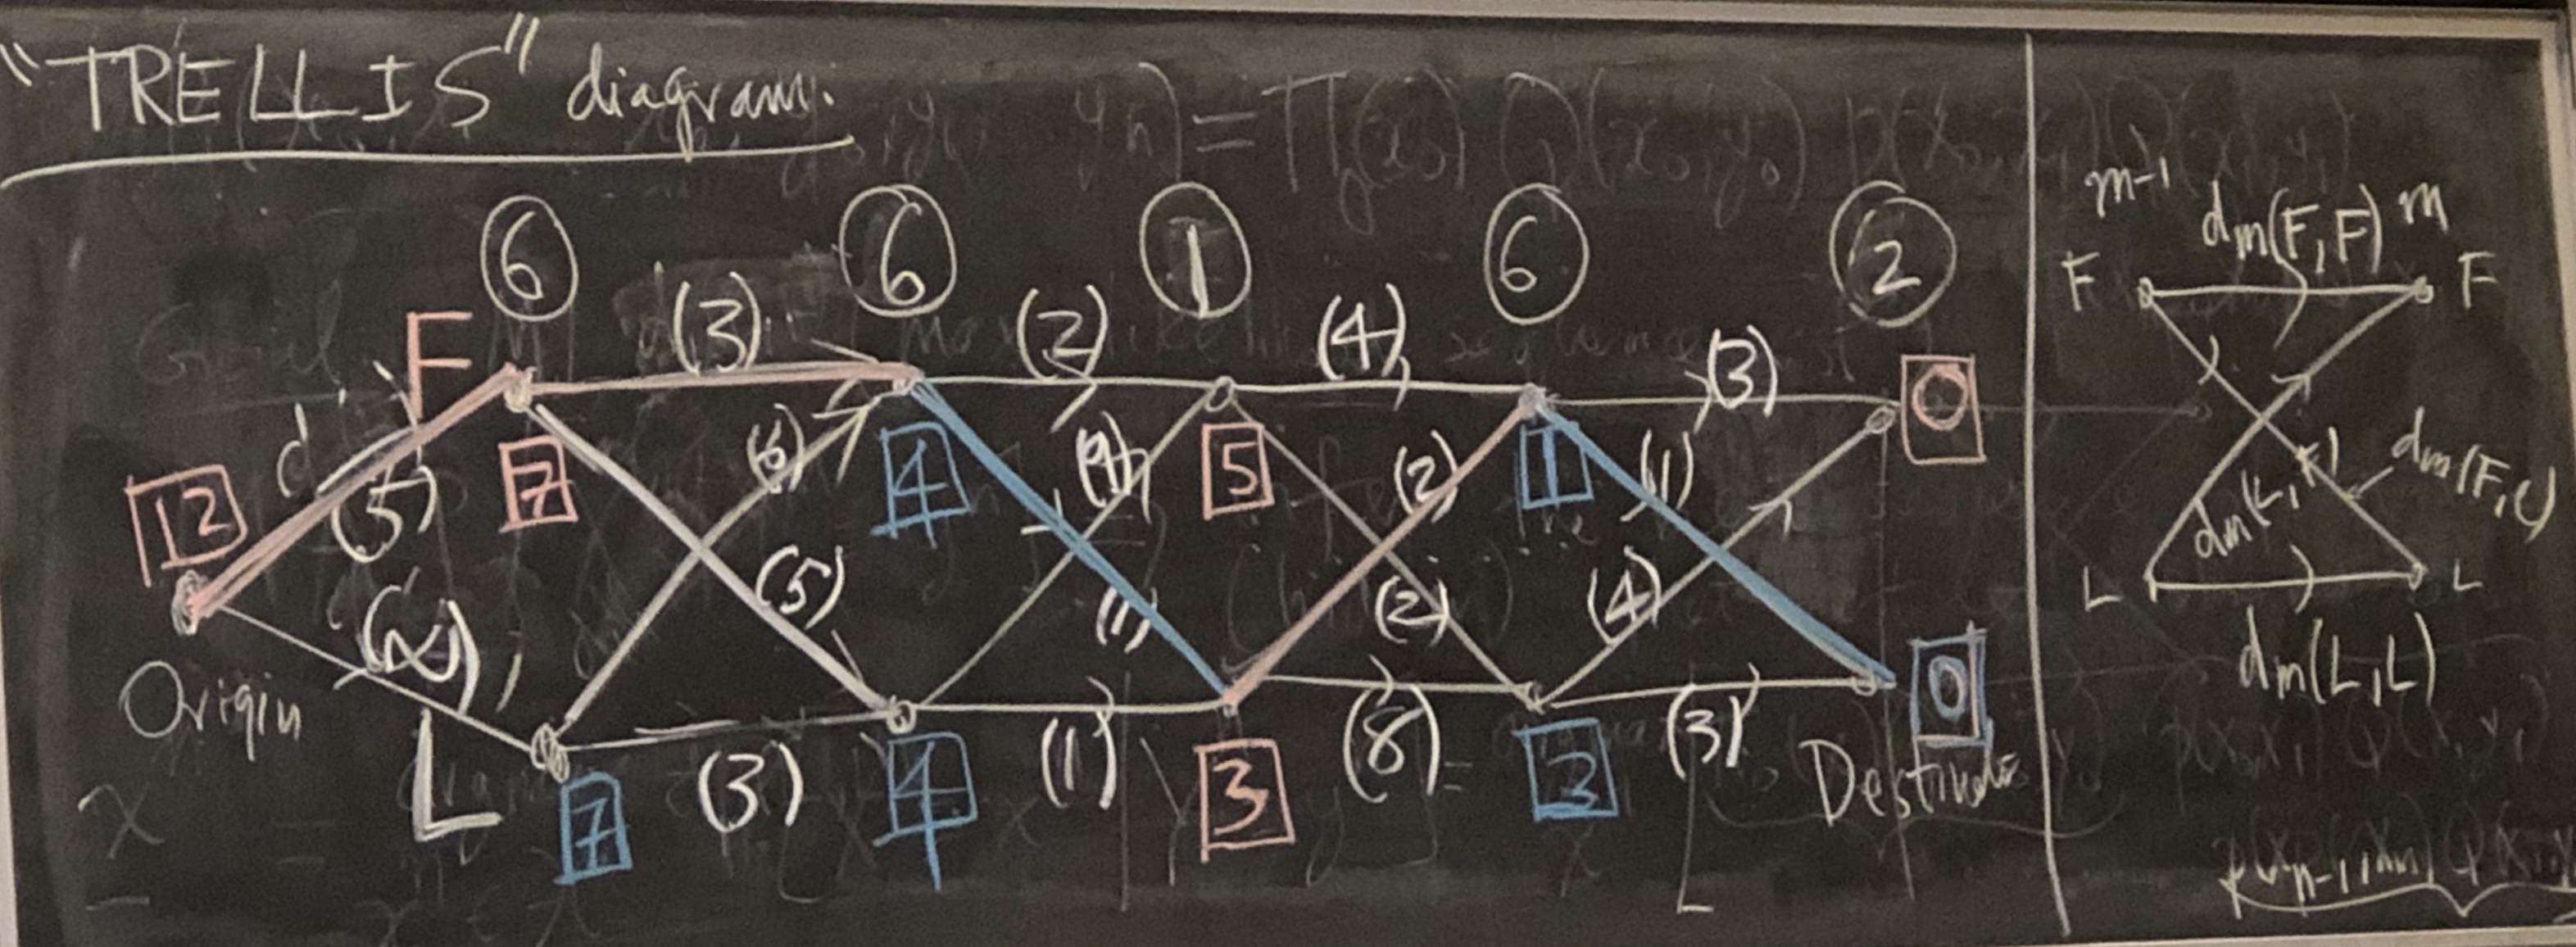
\includegraphics[scale=0.13]{trellis_complete.jpg}
    \caption{The TRELLIS diagram filled in with edge weights and the shortest path.}
\end{figure}

The circled numbers are the observations, and the numbers along every edge are the weights. The boxed numbers are the shortest path values from that node to the final stage; blue numbers represent transitions to a loaded die, while red numbers represent transitions to a fair die. Our initial transition from the origin to $L$ is infinity because we're told that the casino will start with a fair die. 

If we work our way back through this diagram, we can find that the MLSE estimate is $(F, F, L, F, L)$. 

Finally, we can do a quick analysis of how much time each of these methods take. The cost of populating trellis is $O(N^2 n)$ where $N$ is the number of states and $n$ is the number of stages. If we have a populated trellis, it only takes $O(Nn)$ to find the shortest path (since we only have one node at each stage to consider). Note that the naive completion is just $O(N^n)$, so we're doing really well. We turned a computational infeasible problem into a pretty efficient one. 

\end{document}
